\chapter{泛函分析与逼近理论}
\label{chap:functional-analysis-and-approximation}

有限维模型常把函数写成固定基函数的线性组合：
\begin{equation}
  f_m(x)=\sum_{j=1}^{m}a_j\phi_j(x).
  \label{eq:functional-finite-basis-expansion}
\end{equation}
当$m$固定时，可以把系数$(a_1,\ldots,a_m)^{\top}$当作普通向量，用欧氏距离比较两个
候选解。然而，一旦允许基函数数目增加，系数向量所在的维数也随之改变；同一个函数还可能
在不同基下拥有完全不同的系数。此时，仅比较参数向量已经不能稳定地回答三个问题：函数
之间相差多少，有限表示能否逼近目标，以及从数据选择出的函数有多复杂。

本章改为直接把函数看成空间中的点。范数规定误差怎样度量，完备性保证逼近序列的极限仍在
空间内，内积则把有限维最小二乘中的正交与投影推广到函数。若还要求能够连续地读取函数在
某个输入处的值，就会得到再生核Hilbert空间（reproducing kernel Hilbert space, RKHS）。
核谱在选定测度后解释全域方向与正则化尺度。在此基础上，再区分表示能力与函数类大小：前者问某个目标能否被逼近，后者问候选函数
可以沿多少方向、以多细尺度变化。这一区分将在后续概率章节中进入有限观测误差，但本章只
建立其中不依赖随机抽样的空间结构。

\section{函数作为空间中的对象}
\label{sec:functional-functions-as-space-elements}

\subsection{函数空间的线性结构}

设$\mathcal{X}$为输入集合，$\mathbb{R}^{\mathcal{X}}$表示从$\mathcal{X}$到
$\mathbb{R}$的全部函数。对$f,g\in\mathbb{R}^{\mathcal{X}}$和$a,b\in\mathbb{R}$，
定义
\[
  (af+bg)(x)=af(x)+bg(x),\qquad x\in\mathcal{X}.
\]
这些逐点运算使$\mathbb{R}^{\mathcal{X}}$成为向量空间。式
\eqref{eq:functional-finite-basis-expansion}描述的集合只是其中由
$\phi_1,\ldots,\phi_m$张成的有限维子空间。允许无限多个基方向以后，线性结构仍然
存在，但坐标数目不再适合作为唯一的大小尺度。

函数可以相加，并不表示已经知道两个函数相差多少。把误差汇总成一个非负数，还要要求
缩放与累加时的误差具有一致规则；这正是范数的作用。
\begin{definition}[赋范空间]
\label{def:functional-normed-space}
设$\mathcal V$为实向量空间。映射$\lVert\cdot\rVert_{\mathcal V}:\mathcal V\to[0,\infty)$
若对任意$f,g\in\mathcal V$和$a\in\mathbb R$满足
\[
  \lVert f\rVert_{\mathcal{V}}\geq0,\qquad
  \lVert f\rVert_{\mathcal{V}}=0\Longleftrightarrow f=0,\qquad
  \lVert af\rVert_{\mathcal{V}}=|a|\lVert f\rVert_{\mathcal{V}},
\]
以及三角不等式
$\lVert f+g\rVert_{\mathcal{V}}\leq
\lVert f\rVert_{\mathcal{V}}+\lVert g\rVert_{\mathcal{V}}$。
则称为范数，$(\mathcal V,\lVert\cdot\rVert_{\mathcal V})$称为\term{赋范空间}
（normed space）。它诱导距离$d(f,g)=\lVert f-g\rVert_{\mathcal V}$。
\end{definition}
选择不同范数，就是选择不同的误差含义。范数必须为每个空间元素给出有限值；因此，
选定积分范数后，还要把不满足相应可积条件的函数排除在空间之外。

例如，紧区间$[a,b]$上的连续函数空间$C([a,b])$常使用一致范数
\[
  \lVert f\rVert_{\infty}
  =\sup_{x\in[a,b]}|f(x)|.
\]
这个范数控制每个输入上的最大误差。若$\mu$是一个测度，则第
\ref{chap:mathematical-analysis}章建立的$L^p(\mu)$空间使用
\[
  \lVert f\rVert_{L^p(\mu)}
  =
  \left(\int_{\mathcal{X}}|f(x)|^p\,\mathrm{d}\mu(x)\right)^{1/p},
  \qquad 1\leq p<\infty.
\]
它控制的是相对于$\mu$的整体误差，允许函数在小测度集合上偏离较大。两种误差不能互相
替代：在$[0,1]$上令
\[
  f_n(x)=\max\{1-nx,0\},
\]
则$\lVert f_n\rVert_{L^2}^2=1/(3n)\to0$，但
$\lVert f_n\rVert_{\infty}=1$始终不变。

\begin{figure}[htbp]
 \centering
 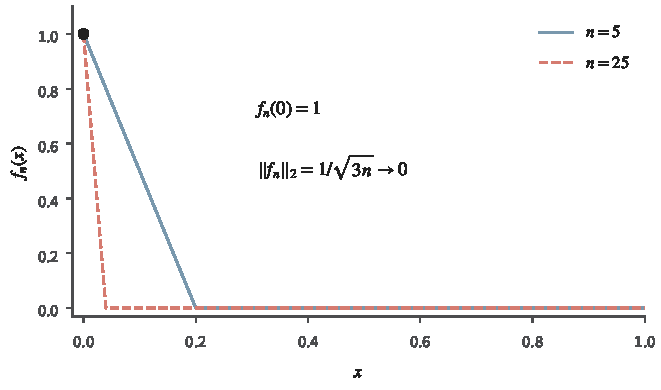
\includegraphics[width=\linewidth]{figures/math-preparation/analysis-geometry/functional-point-evaluation.pdf}
 \caption{连续尖峰$f_n(x)=\max\{1-nx,0\}$在$L^2$范数下趋于零，原点函数值却始终为$1$。峰宽分别为$1/5$和$1/25$；蓝、红线均由解析式生成。整体能量控制不等于稳定的点值控制。}
 \label{fig:functional-point-evaluation}
\end{figure}

后面的完备性证明会用到$L^2$版本的\term{Minkowski不等式}
（Minkowski inequality），也就是$L^2$范数的三角不等式。对$f,g\in L^2(\mu)$，
Cauchy--Schwarz不等式给出
\[
  \begin{aligned}
  \lVert f+g\rVert_{L^2(\mu)}^2
  &=
  \lVert f\rVert_{L^2(\mu)}^2
  +
  2\int_{\mathcal{X}}f(x)g(x)\,\mathrm{d}\mu(x)
  +\lVert g\rVert_{L^2(\mu)}^2\\
  &\leq
  \bigl(
    \lVert f\rVert_{L^2(\mu)}
    +
    \lVert g\rVert_{L^2(\mu)}
  \bigr)^2.
  \end{aligned}
\]
两边开平方便得到
$\lVert f+g\rVert_{L^2(\mu)}
\leq\lVert f\rVert_{L^2(\mu)}+\lVert g\rVert_{L^2(\mu)}$；
反复使用即可控制有限个函数之和。

\subsection{Banach空间与完备性}

不断增加基函数时，可能得到越来越接近的候选函数，却始终没有一个有限表示等于极限。
分析章的完备性在这里要求：这些候选若按所选范数形成柯西序列，空间就应容纳它们的极限。
\begin{definition}[Banach空间]
\label{def:functional-banach-space}
若赋范空间$\mathcal V$在诱导距离$d(f,g)=\lVert f-g\rVert_{\mathcal V}$下完备，
即每个范数柯西序列都在该范数下收敛到$\mathcal V$中的元素，则称其为
\term{Banach空间}（Banach space）。
\end{definition}
完备性不负责证明某个具体
序列是柯西序列；它只保证一旦误差足以让序列内部彼此靠近，极限不会落到空间之外。

区间$[a,b]$上的$C([a,b])$配备一致范数是Banach空间。事实上，若$(f_n)$在一致范数
下为柯西序列，那么每个$x$处的$(f_n(x))$都是实数柯西序列，可以定义
$f(x)=\lim_n f_n(x)$。柯西条件对所有$x$使用同一个$N$，故$f_n$一致收敛到$f$；
连续函数的一致极限仍连续，所以$f\in C([a,b])$。

同一个函数集合换一种范数可能失去完备性。连续函数空间$C([0,1])$配备$L^2$范数就
不是完备的。取连续函数$f_n$逐渐逼近阶跃函数
$\mathbb{I}\{x>1/2\}$，可以使$(f_n)$在$L^2$中为柯西序列，但它的$L^2$极限没有
任何处处连续的代表元。完成这个空间需要加入可测函数的几乎处处等价类，得到
$L^2([0,1])$。这里“几乎处处等价”很关键：如果$f$与$g$只在零测集上不同，它们在
$L^2$中是同一个元素。

$L^2(\mu)$本身的完备性可以从柯西列内部构造极限。设$(f_n)$在$L^2(\mu)$中为
柯西列。逐次选取子列$(f_{n_k})$，使
\[
  \lVert f_{n_{k+1}}-f_{n_k}\rVert_{L^2(\mu)}
  \leq 2^{-k}.
\]
令$h_k=|f_{n_{k+1}}-f_{n_k}|$。对有限部分和反复使用上面的$L^2$版Minkowski
不等式，再用Fatou引理，可得
\[
  \int_{\mathcal{X}}
  \left(\sum_{k=1}^{\infty}h_k\right)^2
  \,\mathrm{d}\mu
  \leq
  \left(\sum_{k=1}^{\infty}2^{-k}\right)^2
  <\infty.
\]
因此$\sum_k h_k(x)$几乎处处有限，$(f_{n_k}(x))$在这些点绝对收敛。把它的几乎处处
极限记为$f$。同样对尾和使用Fatou引理，得到
\[
  \lVert f_{n_\ell}-f\rVert_{L^2(\mu)}
  \leq
  \sum_{k=\ell}^{\infty}2^{-k}
  \longrightarrow0.
\]
原序列是柯西列，故它与已收敛子列的距离也趋于零，从而$f_n\to f$于$L^2(\mu)$。
这个论证同时说明为何要把只在零测集上不同的代表元视为同一元素：构造得到的点态极限
本来就只在几乎处处意义下确定。对$1\leq p<\infty$可用相同的可求和子列思路证明
$L^p(\mu)$完备；$p=\infty$时则控制本质上确界。因此，$1\leq p\leq\infty$时的
$L^p(\mu)$都是Banach空间，而$L^2(\mu)$还具有下面要用的内积结构。

\subsection{Hilbert空间与内积}

范数给出长度和距离，却未必能定义夹角。要把最小二乘的正交残差推广到函数，需要再加入
能够比较两个方向的内积。
\begin{definition}[实内积空间与Hilbert空间]
\label{def:functional-hilbert-space}
\term{内积空间}（inner-product space）在实向量空间$\mathcal{V}$上配备对称双线性
映射$\langle\cdot,\cdot\rangle_{\mathcal{V}}:\mathcal V\times\mathcal V\to\mathbb R$，并要求
$\langle f,f\rangle_{\mathcal{V}}>0$对每个非零$f$成立。内积诱导范数
\[
  \lVert f\rVert_{\mathcal{V}}
  =\sqrt{\langle f,f\rangle_{\mathcal{V}}}.
\]
相应范数下完备的内积空间称为\term{Hilbert空间}（Hilbert space）。
\end{definition}
它把欧氏空间中
长度、夹角、正交和投影的关系保留下来，同时允许空间无限维。

$L^2(\mu)$是基本例子，其内积为
\[
  \langle f,g\rangle_{L^2(\mu)}
  =\int_{\mathcal{X}}f(x)g(x)\,\mathrm{d}\mu(x).
\]
但$L^1(\mu)$与一般的$L^p(\mu)$并不都由内积诱导。一个范数来自内积，当且仅当它满足
\term{平行四边形恒等式}（parallelogram identity）
\begin{equation}
  \lVert f+g\rVert^2+\lVert f-g\rVert^2
  =
  2\lVert f\rVert^2+2\lVert g\rVert^2.
  \label{eq:functional-parallelogram-identity}
\end{equation}
例如在$\mathbb{R}^2$的$L^1$范数中取
$\bm{u}=(1,0)^{\top}$、$\bm{v}=(0,1)^{\top}$，左侧为$8$，右侧为$4$，所以这个
范数不可能来自内积。Banach空间提供极限与距离，Hilbert空间额外提供正交几何；后面的
投影结论依赖后者，不能只靠完备范数得到。

无限维还使一些有限维中自动成立的性质需要单独检查。有限维子空间总是闭集，有界序列总能
抽出收敛子列，线性映射也自动连续；这些陈述在一般无限维空间中都可能失效。例如
$\ell^2$中的标准单位向量$(\bm{e}_j)_{j\geq1}$都位于单位球内，但$j\neq k$时
\[
  \lVert\bm{e}_j-\bm{e}_k\rVert_2=\sqrt{2}.
\]
这个序列没有柯西子列，因而也没有收敛子列。无限维闭单位球由此给出“闭且有界未必紧”
的具体反例；这里具体指$\ell^2$的闭单位球。

有限表示可能并未包含极限，却能任意接近它；这项逼近性质应与空间的完备性分开。
\begin{definition}[稠密子集]
\label{def:functional-density}
设$(\mathcal V,\lVert\cdot\rVert)$为赋范空间，$\mathcal F\subseteq\mathcal V$。
若对每个$f\in\mathcal V$和每个$\varepsilon>0$，存在$g\in\mathcal F$满足
$\lVert f-g\rVert<\varepsilon$，则称$\mathcal F$在$\mathcal V$中稠密。
等价地，$\mathcal F$在该范数诱导距离下的闭包等于$\mathcal V$。
\end{definition}
这里的闭包由原集合及所有能被它任意接近的点组成；稠密不要求这些点已属于$\mathcal F$。
完备性与稠密性也不能混为一谈。
$\ell^2$由平方可和序列$\bm{a}=(a_1,a_2,\ldots)$组成，范数为
$\lVert\bm{a}\rVert_2^2=\sum_{j=1}^{\infty}a_j^2$。只有有限个非零坐标的序列构成
子空间$c_{00}$，它在$\ell^2$中稠密却不闭。序列
$(1,1/2,\ldots,1/n,0,\ldots)$属于$c_{00}$，其极限
$(1,1/2,1/3,\ldots)$属于$\ell^2$但不属于$c_{00}$。这正是闭性在最佳逼近问题中
不能省略的原因。有限截断能够不断逼近$\ell^2$中的元素，说明$c_{00}$的闭包是
$\ell^2$；它并不说明$c_{00}$自身已经包含这些极限。

\section{正交展开与函数投影}
\label{sec:functional-orthogonal-expansions-projections}

范数空间允许比较函数并取极限，内积空间还可以辨认正交方向。
本节把有限维最小二乘中的最近点问题推广到函数空间：闭性、凸性和完备性分别保证可行极限、
唯一最近点和极限存在。正交展开由此获得误差分解，其有效性还取决于所选方向是否张成目标。

\subsection{闭凸集上的最近点}

有限维最小二乘把观测向量投影到设计矩阵的列空间。函数逼近的对应问题是：给定Hilbert
空间$\mathcal{H}$中的目标$f$与候选集合$C$，能否找到$g^\star\in C$使
$\lVert f-g^\star\rVert_{\mathcal{H}}$最小？下面的投影定理中，非空性只保证距离
下确界有候选可比较；凸性与内积几何先使最小化序列成为柯西列，Hilbert空间的完备性
保证该序列在空间中有极限，闭性再把极限留在$C$内。凸性还参与唯一性与变分不等式的
证明，因而不能把四项条件各自简化成互不相干的一项职责。

\begin{theorem}[Hilbert空间投影定理]
\label{thm:functional-hilbert-projection}
设$\mathcal{H}$为实Hilbert空间，$C\subseteq\mathcal{H}$非空、闭且凸。对每个
$f\in\mathcal{H}$，存在唯一的$g^\star\in C$满足
\[
  \lVert f-g^\star\rVert_{\mathcal{H}}
  =\inf_{g\in C}\lVert f-g\rVert_{\mathcal{H}}.
\]
这个最近点由变分不等式
\begin{equation}
  \langle f-g^\star,g-g^\star\rangle_{\mathcal{H}}
  \leq0,\qquad g\in C
  \label{eq:functional-convex-projection-characterization}
\end{equation}
唯一刻画。若$C=M$是闭线性子空间，则该条件等价于
\begin{equation}
  f-g^\star\perp M.
  \label{eq:functional-subspace-projection-orthogonality}
\end{equation}
\end{theorem}

\begin{proof}
记$d=\inf_{g\in C}\lVert f-g\rVert_{\mathcal{H}}$，并取最小化序列
$(g_n)\subseteq C$，使$\lVert f-g_n\rVert_{\mathcal{H}}\to d$。凸性保证
$(g_n+g_m)/2\in C$。把平行四边形恒等式用于
$f-g_n$与$f-g_m$，得到
\begin{align*}
  \lVert g_n-g_m\rVert_{\mathcal{H}}^2
  &=
  2\lVert f-g_n\rVert_{\mathcal{H}}^2
  +2\lVert f-g_m\rVert_{\mathcal{H}}^2\\
  &\quad
  -4\left\lVert
    f-\frac{g_n+g_m}{2}
  \right\rVert_{\mathcal{H}}^2\\
  &\leq
  2\lVert f-g_n\rVert_{\mathcal{H}}^2
  +2\lVert f-g_m\rVert_{\mathcal{H}}^2-4d^2.
\end{align*}
右侧随$m,n\to\infty$趋于$0$，所以$(g_n)$是柯西序列。$\mathcal{H}$完备，故
$g_n\to g^\star\in\mathcal{H}$；$C$闭，故$g^\star\in C$。范数连续给出
$\lVert f-g^\star\rVert_{\mathcal{H}}=d$，存在性得证。

若$g_1,g_2\in C$都达到$d$，同一恒等式给出
\[
  \lVert g_1-g_2\rVert_{\mathcal{H}}^2
  =
  2d^2+2d^2
  -4\left\lVert f-\frac{g_1+g_2}{2}\right\rVert_{\mathcal{H}}^2
  \leq0,
\]
所以$g_1=g_2$。

再证明刻画。对任意$g\in C$和$t\in[0,1]$，凸性给出
$g^\star+t(g-g^\star)\in C$。最优性意味着
\[
  \lVert f-g^\star\rVert_{\mathcal{H}}^2
  \leq
  \lVert f-g^\star-t(g-g^\star)\rVert_{\mathcal{H}}^2.
\]
展开右侧、约去公共项并除以$t>0$，得到
\[
  2\langle f-g^\star,g-g^\star\rangle_{\mathcal{H}}
  \leq t\lVert g-g^\star\rVert_{\mathcal{H}}^2.
\]
令$t\downarrow0$便得到式
\eqref{eq:functional-convex-projection-characterization}。反过来，若该不等式成立，
则对任意$g\in C$，
\[
  \lVert f-g\rVert_{\mathcal{H}}^2
  =
  \lVert f-g^\star\rVert_{\mathcal{H}}^2
  +\lVert g-g^\star\rVert_{\mathcal{H}}^2
  -2\langle f-g^\star,g-g^\star\rangle_{\mathcal{H}}
  \geq
  \lVert f-g^\star\rVert_{\mathcal{H}}^2,
\]
所以$g^\star$是最近点。

若$C=M$为线性子空间，则对每个$h\in M$，可分别取
$g=g^\star+h$和$g=g^\star-h$。式
\eqref{eq:functional-convex-projection-characterization}同时给出
$\langle f-g^\star,h\rangle\leq0$与
$-\langle f-g^\star,h\rangle\leq0$，故内积为零。反向结论由勾股恒等式直接得到。
\end{proof}

闭性不能由“子空间”二字自动获得。以前面的$c_{00}\subset\ell^2$为例，目标
$\bm{a}=(1,1/2,1/3,\ldots)$到$c_{00}$的距离下确界为$0$，但$\bm{a}\notin c_{00}$，
所以不存在最佳逼近。有限截断可以任意接近目标，却没有一个有限截断达到距离$0$。

\subsection{正交展开与误差分解}

为了逐方向读出系数，需要先固定这些方向是否独立，以及是否遗漏其他方向。
\begin{definition}[正交归一序列与完备正交系]
\label{def:functional-complete-orthonormal-system}
设$\mathcal H$为Hilbert空间。序列$(e_j)_{j\geq1}$若满足
$\langle e_j,e_k\rangle_{\mathcal H}=\mathbb I\{j=k\}$，称为正交归一序列。
若它的有限线性张成在$\mathcal H$中稠密，则称为\term{完备正交系}
（complete orthonormal system）。
\end{definition}
有限维时同样使用有限序列；“完备”要求覆盖空间的全部方向。
目标$f$在前$m$个方向上的
投影为
\begin{equation}
  P_m f
  =
  \sum_{j=1}^{m}
  \langle f,e_j\rangle_{\mathcal{H}}e_j.
  \label{eq:functional-orthogonal-partial-projection}
\end{equation}
因为$f-P_mf$与每个$e_j$正交，定理
\ref{thm:functional-hilbert-projection}说明$P_mf$是
$\operatorname{span}\{e_1,\ldots,e_m\}$中的唯一最佳逼近。勾股恒等式进一步给出
\begin{equation}
  \lVert f-P_mf\rVert_{\mathcal{H}}^2
  =
  \lVert f\rVert_{\mathcal{H}}^2
  -
  \sum_{j=1}^{m}
  |\langle f,e_j\rangle_{\mathcal{H}}|^2.
  \label{eq:functional-projection-error-decomposition}
\end{equation}
左侧非负，于是得到Bessel不等式
$\sum_{j\geq1}|\langle f,e_j\rangle|^2\leq\lVert f\rVert^2$。
定义~\ref{def:functional-complete-orthonormal-system}中的完备性等价于：若
$f\in\mathcal{H}$与每个$e_j$都正交，则$f=0$。此时$P_mf\to f$，上式成为Parseval
恒等式。“系数可平方求和”与“展开恢复整个函数”之间差的正是所选正交系是否完备，也就是
它是否遗漏了与所有$e_j$正交的非零方向。

正交系的完备性与Hilbert空间的完备性不是同一性质。前者考察一组给定方向能否稠密张成
整个空间，后者考察任意柯西序列的极限是否仍在空间内。例如$\ell^2$是完备的Hilbert
空间，但只取$(\bm{e}_{2j})_{j\geq1}$会遗漏所有奇数坐标方向，因此这组正交归一向量
不是完备正交系。

\subsection{加权函数投影}

设$w$是$[-1,1]$上可测、几乎处处为正且属于$L^1([-1,1])$的权重。在关于测度
$w(x)\,\mathrm{d}x$的几乎处处等价类所成空间
$L^2([-1,1],w(x)\,\mathrm{d}x)$上，定义
\[
  \langle f,g\rangle_w
  =
  \int_{-1}^{1}f(x)g(x)w(x)\,\mathrm{d}x.
\]
加权平方可积性与Cauchy--Schwarz不等式保证该积分对空间中任意$f,g$有限；权重几乎
处处为正则保证它确实定义内积。由于紧区间上的多项式有界，而$w$可积，每个多项式都属于
这个加权空间，因此可以对幂函数序列作Gram--Schmidt正交化。权重$w(x)=1$对应Legendre
多项式；权重$w(x)=(1-x^2)^{-1/2}$（端点值任取）对应第一类Chebyshev多项式
$T_j(x)=\cos(j\arccos x)$。后者在$x=\pm1$附近赋予更大权重，因此相同次数的投影
优化的是另一种积分误差。

只保留计算展开所需的低阶关系即可。Legendre多项式满足
\[
  P_0(x)=1,\qquad P_1(x)=x,\qquad
  (j+1)P_{j+1}(x)=(2j+1)xP_j(x)-jP_{j-1}(x),
\]
Chebyshev多项式满足
\[
  T_0(x)=1,\qquad T_1(x)=x,\qquad
  T_{j+1}(x)=2xT_j(x)-T_{j-1}(x).
\]
这些递推生成的是相对于各自权重正交的方向，而不是同一组多项式换了名称。

对$f(x)=x^2$，只用$\operatorname{span}\{1,x\}$逼近时，对称权重使一次项系数为零。
最佳常数为$\langle x^2,1\rangle_w/\langle1,1\rangle_w$：均匀权重给出
$\frac{\int_{-1}^1x^2\,\mathrm dx}{\int_{-1}^1\mathrm dx}=1/3$，Chebyshev权重经
$x=\cos\theta$换元则给出
$\frac{\int_0^\pi\cos^2\theta\,\mathrm d\theta}{\int_0^\pi\mathrm d\theta}=1/2$。
后者更重视两端，而$f$恰在两端较大，故最佳常数也随之增大。

图~\ref{fig:functional-weighted-projection}把两条最佳常数放在同一个目标上比较。
选择相同的候选空间还不够；权重改变后，“最近”的含义已经改变。不能把一次投影的
结果脱离其内积，称为不加限定的最佳逼近。
\begin{figure}[htbp]
 \centering
 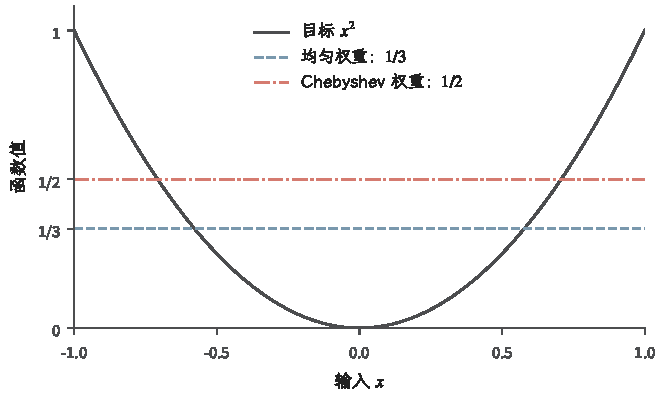
\includegraphics[width=\linewidth]{figures/math-preparation/concept-revision-analysis-functional/weighted-projection.pdf}
 \caption{对$x^2$使用同一候选空间$\operatorname{span}\{1,x\}$，均匀权重的最佳常数为$1/3$，Chebyshev权重的最佳常数为$1/2$。目标、区间和候选空间保持相同，只改变误差积分的权重。曲线由解析式生成。}
 \label{fig:functional-weighted-projection}
\end{figure}

区间或权重改变后，正交系数必须随之重算。把$[a,b]$仿射映射到$[-1,1]$可以迁移
Legendre或Chebyshev基，但Jacobian因子和权重也会改变。Chebyshev多项式还具有适合
一致逼近与插值的极值分布；这不意味着其加权$L^2$投影自动就是一致范数下的最佳逼近。
投影结论始终相对于所选内积成立，误差度量一旦改变，最佳函数也可能改变。

\subsection{稳定读取与内积表示}

对函数取加权积分、读出一个系数或在一点求值，都会把整条函数变成一个数。要判断这些
读取操作是否稳定，需检查输入函数的小范数误差能否控制输出误差。
\begin{definition}[有界线性泛函]
\label{def:functional-bounded-linear-functional}
设$\mathcal V$为实赋范空间。线性泛函是线性映射$L:\mathcal V\to\mathbb R$。
若存在有限常数$C\geq0$，使
$|L(f)|\leq C\lVert f\rVert_{\mathcal V}$对所有$f\in\mathcal V$成立，则称$L$有界。
\end{definition}
有界不是要求$L$在整个空间中的输出有统一上限，而是要求输出大小相对于输入范数有
统一上限。线性性使$|L(f)-L(g)|\leq C\lVert f-g\rVert$；在赋范空间上，线性泛函
的有界性与连续性等价。Hilbert空间的内积给出一类直接的有界泛函：
$L_h(f)=\langle f,h\rangle_{\mathcal{H}}$。Riesz表示定理说明没有别的有界线性
泛函\scite{math-conway1990functional}

\begin{theorem}[Riesz表示定理]
\label{thm:functional-riesz-representation}
设$\mathcal{H}$为实Hilbert空间。对每个有界线性泛函
$L:\mathcal{H}\to\mathbb{R}$，存在唯一的$h_L\in\mathcal{H}$，使
\begin{equation}
  L(f)=\langle f,h_L\rangle_{\mathcal{H}},
  \qquad f\in\mathcal{H}.
  \label{eq:functional-riesz-representation}
\end{equation}
并且$\lVert L\rVert=\lVert h_L\rVert_{\mathcal{H}}$，其中
$\lVert L\rVert=\sup_{\lVert f\rVert_{\mathcal{H}}\leq1}|L(f)|$。
\end{theorem}

\begin{proof}
若$L=0$，取$h_L=0$即可。以下设$L\neq0$。核空间
$M=\ker L=\{f:L(f)=0\}$是线性子空间；由于$L$连续，$M$也是闭集。选取
$u\in\mathcal{H}$使$L(u)\neq0$。由定理
\ref{thm:functional-hilbert-projection}，可以把$u$唯一分解为
\[
  u=P_Mu+v,\qquad v\in M^\perp.
\]
若$v=0$，则$u\in M$，与$L(u)\neq0$矛盾，故$v\neq0$。
又因$P_Mu\in M=\ker L$，
\[
  L(v)=L(u)-L(P_Mu)=L(u)\neq0,
\]
所以下面的除法合法。

对任意$f\in\mathcal{H}$，向量
\[
  f-\frac{L(f)}{L(v)}v
\]
的$L$值为零，因而属于$M$。它与$v\in M^\perp$正交，所以
\[
  0
  =
  \left\langle
    f-\frac{L(f)}{L(v)}v,v
  \right\rangle_{\mathcal{H}}
  =
  \langle f,v\rangle_{\mathcal{H}}
  -
  \frac{L(f)}{L(v)}\lVert v\rVert_{\mathcal{H}}^2.
\]
整理得到
\[
  L(f)
  =
  \left\langle
    f,\frac{L(v)}{\lVert v\rVert_{\mathcal{H}}^2}v
  \right\rangle_{\mathcal{H}}.
\]
因此可取
$h_L=L(v)v/\lVert v\rVert_{\mathcal{H}}^2$。

若$h_1,h_2$都表示$L$，则
$\langle f,h_1-h_2\rangle=0$对每个$f$成立。取$f=h_1-h_2$便得
$h_1=h_2$。Cauchy--Schwarz不等式给出
$|L(f)|\leq\lVert f\rVert\lVert h_L\rVert$，所以
$\lVert L\rVert\leq\lVert h_L\rVert$；当$h_L\neq0$时取
$f=h_L/\lVert h_L\rVert$得到反向不等式。$h_L=0$的情形也直接成立。
\end{proof}

有时读取结果仍是一个函数，例如把一个函数空间映入另一个函数空间。
此时要比较输出与某个测试方向的内积，就需要把这个测试方向拉回输入空间。
\begin{definition}[Hilbert空间之间的伴随算子]
\label{def:functional-adjoint}
设$\mathcal H,\mathcal G$为实Hilbert空间，$S:\mathcal H\to\mathcal G$为有界线性算子，
即存在有限$C\geq0$使$\lVert Sf\rVert_{\mathcal G}\leq C\lVert f\rVert_{\mathcal H}$。
其伴随是满足
\[
 \langle Sf,g\rangle_{\mathcal G}
 =\langle f,S^*g\rangle_{\mathcal H}
 \quad(f\in\mathcal H,\ g\in\mathcal G)
\]
的有界线性算子$S^*:\mathcal G\to\mathcal H$。
\end{definition}
对固定$g$，左边是关于$f$的有界线性泛函，Riesz表示给出唯一的$S^*g$；
表示元的唯一性又保证$S^*$线性，且$\lVert S^*g\rVert_{\mathcal H}\leq C\lVert g\rVert_{\mathcal G}$。
因此伴随确实存在且唯一。它把内积中的算子换到另一侧，并不要求$S$可逆；
有限维实正交坐标中它对应通常的转置；复内积空间使用相应的复数版本，才对应共轭转置。后面的Mercer证明会对空间之间的
包含映射使用同一概念。

\section{正定核与再生核空间}
\label{sec:functional-positive-kernels-rkhs}

整体误差小未必使每个点的函数值接近，前面的尖峰例子已经说明这一点。
若观测和预测通过点值进行，就需要点值读取相对于空间范数稳定。
前节已为一般稳定读取建立Riesz表示；本节专门考察点值泛函，核由此成为空间中的表示对象，
后面的有限核展开则是优化问题在这个空间内的结果。

\subsection{点值泛函与再生核}

上一小节允许读取任意有界线性泛函。这里专门要求读出$f(x)$，因为有限观测与预测通常
需要访问函数在指定位置的值。
\begin{definition}[再生核Hilbert空间]
\label{def:functional-rkhs}
设$\mathcal X$为非空集合，$\mathcal H\subseteq\mathbb R^{\mathcal X}$是实值函数
Hilbert空间。若对每个$x\in\mathcal X$，点值泛函$\delta_x(f)=f(x)$均有界，
则称$\mathcal H$为\term{再生核Hilbert空间}。
\end{definition}
定义要求空间元素是真正具有确定点值的函数。不同的$x$可以使用不同的有界常数；
它并没有要求$x\mapsto f(x)$在某种输入拓扑下连续。
Riesz表示定理给出唯一元素$K_x\in\mathcal{H}$，使
\begin{equation}
  f(x)=\langle f,K_x\rangle_{\mathcal{H}},
  \qquad f\in\mathcal{H}.
  \label{eq:functional-reproducing-property}
\end{equation}
定义
\[
  K(x,z)=K_z(x)
  =\langle K_z,K_x\rangle_{\mathcal{H}},
\]
便得到空间的\term{再生核}（reproducing kernel）。式
\eqref{eq:functional-reproducing-property}说明“再生”的含义：函数在$x$处的值可以
由函数与核截面$K_x=K(\,\cdot\,,x)$的内积读出。

普通$L^2(\mu)$通常不是RKHS。其元素是几乎处处等价类，在单个点上改值不改变元素，
所以$f(x)$甚至未必定义良好。即使人为选择代表元，点值也一般不连续：在$[0,1]$上可以
构造支撑越来越窄而在固定点取值为$1$的连续尖峰，其$L^2$范数趋于$0$。因此，从
$L^2$收敛不能推出固定点的函数值收敛。RKHS范数额外控制点值，因为
\begin{equation}
  |f(x)|
  \leq
  \lVert f\rVert_{\mathcal{H}}
  \lVert K_x\rVert_{\mathcal{H}}
  =
  \lVert f\rVert_{\mathcal{H}}\sqrt{K(x,x)}.
  \label{eq:functional-rkhs-pointwise-bound}
\end{equation}

输入之间的核值也不能随意指定：必须让任何有限线性组合的平方长度非负。
\begin{definition}[实正定核]
\label{def:functional-positive-definite-kernel}
设$\mathcal X$非空。对称函数$K:\mathcal X\times\mathcal X\to\mathbb R$若对每个
$n\geq1$、任意$x_1,\ldots,x_n\in\mathcal X$和$a_1,\ldots,a_n\in\mathbb R$都满足
$\sum_{i,j=1}^n a_i a_jK(x_i,x_j)\geq0$，则称其为\term{正定核}
（positive definite kernel）。本章采用核理论中允许半正定的命名惯例。
\end{definition}
从再生性质得到的核满足这个条件，因为
\begin{equation}
  \sum_{i,j=1}^{n}a_i a_jK(x_i,x_j)
  =
  \left\lVert\sum_{i=1}^{n}a_iK_{x_i}\right\rVert_{\mathcal{H}}^2
  \geq0.
  \label{eq:functional-positive-definite-kernel}
\end{equation}
这里沿用核理论的惯例，“正定”允许有限Gram矩阵奇异；若非零系数和互异输入总使二次型
严格为正，才称严格正定。

正定核的一个可直接核验的来源是有限维特征内积。给定映射
$\bm{\phi}:\mathcal{X}\to\mathbb{R}^d$，令
\[
  K_{\bm{\phi}}(x,z)
  =
  \langle\bm{\phi}(x),\bm{\phi}(z)\rangle_2.
\]
对任意有限输入与实系数，
\[
  \sum_{i,j=1}^{n}a_i a_jK_{\bm{\phi}}(x_i,x_j)
  =
  \left\lVert
    \sum_{i=1}^{n}a_i\bm{\phi}(x_i)
  \right\rVert_2^2
  \geq0,
\]
所以$K_{\bm{\phi}}$满足有限半正定条件。例如，当
$\mathcal{X}\subseteq\mathbb{R}$且
$\bm{\phi}(x)=(1,x)^{\top}$时，得到$K_{\bm{\phi}}(x,z)=1+xz$。

\begin{example}[二维函数空间中的再生核]
\label{ex:functional-affine-rkhs}
令$\mathcal X=[-1,1]$，$\mathcal H=\{f(x)=a+bx:a,b\in\mathbb R\}$，
内积为$\langle a+bx,c+dx\rangle=ac+bd$。输入$z$的核截面是
$K_z(x)=1+zx$，因为$\langle a+bx,1+zx\rangle=a+bz=f(z)$。
于是$K(x,z)=1+xz$，$\lVert f\rVert_{\mathcal H}^2=a^2+b^2$，点值上界为
$|f(z)|\leq\sqrt{1+z^2}\sqrt{a^2+b^2}$。

这说明核既可来自有限维空间，也可来自无限维空间。取三个互异输入时，Gram矩阵秩仍至多
为$2$，因为只有两个独立特征方向；核半正定不保证每个有限Gram矩阵都可逆。
表示同一函数的三项核系数可能不唯一，而空间中的函数仍可由严格凸的正则化目标唯一决定。
图~\ref{fig:functional-affine-point-readout}把$f\mapsto f(3/4)$画成系数平面上的读取。
系数圆给出范数上界，平行直线给出相同点值；最远的点值发生在核方向上，
所以点值上界中的$\sqrt{1+z^2}$正是该方向的长度。
\begin{figure}[htbp]
 \centering
 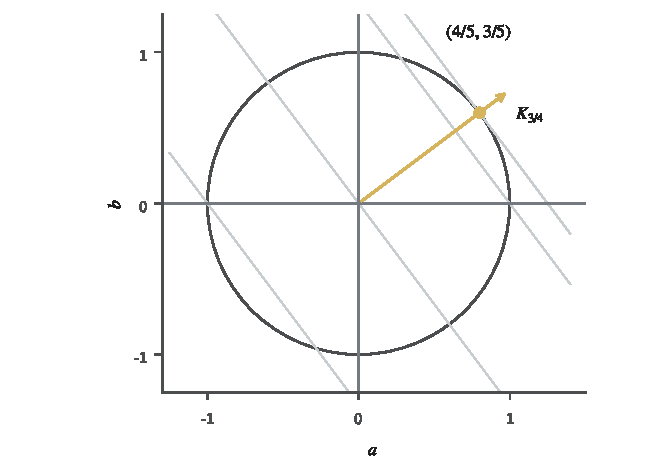
\includegraphics[width=\linewidth]{figures/math-preparation/reader-revision-analysis/functional-affine-point-readout.pdf}
 \caption{仿射RKHS中读取$f(3/4)=a+3b/4$。灰圆表示$a^2+b^2\leq1$，
 黄箭头是核截面$K_{3/4}$对应的系数$(1,3/4)$；灰平行线为相同点值。
 黄圆点$(4/5,3/5)$达到单位范数球上的最大点值$5/4$。这里坐标是函数系数，不是输入位置。图为解析教学示例。}
 \label{fig:functional-affine-point-readout}
\end{figure}

\end{example}

\subsection{Moore--Aronszajn构造}

上面的推导从函数空间得到核。反方向同样成立，而且不需要输入域带有拓扑或测度
\scite{aronszajn1950kernels}

\begin{theorem}[正定核的RKHS构造]
\label{thm:functional-moore-aronszajn-construction}
设$\mathcal{X}$为任意非空集合，$K:\mathcal{X}\times\mathcal{X}\to\mathbb{R}$
对称，并满足式\eqref{eq:functional-positive-definite-kernel}的有限半正定条件。则存在
唯一的函数RKHS $\mathcal{H}_K$以$K$为再生核；这里的唯一性指保持每个函数不变的
等距同构。
\end{theorem}

\begin{proof}
先令$\mathcal{V}_0$为核截面符号$K_x$的形式有限线性组合所成的向量空间：
\[
  \mathcal{V}_0
  =
  \left\{
    \sum_{i=1}^{n}a_iK_{x_i}:
    n\in\mathbb{N},\
    a_i\in\mathbb{R},\
    x_i\in\mathcal{X}
  \right\}.
\]
这里的$K_x$暂时只是由$x$索引的形式符号，尚未把不同形式和按逐点函数值识别。
对
$f=\sum_i a_iK_{x_i}$和$g=\sum_jb_jK_{z_j}$定义
\begin{equation}
  \langle f,g\rangle_0
  =
  \sum_{i,j}a_i b_jK(x_i,z_j).
  \label{eq:functional-kernel-pre-inner-product}
\end{equation}
正定性只保证$\langle f,f\rangle_0\geq0$，还可能有非零形式和的长度为零。令
\[
  \mathcal{N}
  =
  \{f\in\mathcal{V}_0:\langle f,f\rangle_0=0\}.
\]
由半内积的Cauchy--Schwarz不等式，$f\in\mathcal{N}$时
$\langle f,g\rangle_0=0$对所有$g$成立。因此可以商掉$\mathcal{N}$，使式
\eqref{eq:functional-kernel-pre-inner-product}成为真正的内积。

还需证明这个商空间能够忠实地解释为函数。对形式和
$f=\sum_i a_iK_{x_i}$，定义
\[
  (Jf)(x)
  =
  \sum_i a_iK(x,x_i)
  =
  \langle f,K_x\rangle_0.
\]
若$f\in\mathcal{N}$，则
\[
  |(Jf)(x)|^2
  =
  |\langle f,K_x\rangle_0|^2
  \leq
  \langle f,f\rangle_0K(x,x)
  =0,
\]
所以$Jf$处处为零。反过来，若$Jf$处处为零，则
\[
  \langle f,f\rangle_0
  =
  \sum_i a_i(Jf)(x_i)
  =0,
\]
故$f\in\mathcal{N}$。因此$\ker J=\mathcal{N}$，商空间
$\mathcal{H}_0=\mathcal{V}_0/\mathcal{N}$可单射地识别为函数空间，并且其中的
函数满足
\[
  f(x)=\langle f,K_x\rangle_0.
\]

对这个内积空间作完备化，得到Hilbert空间$\mathcal{H}_K$。还要确认完备化后的抽象极限
仍是函数。若$(f_m)\subset\mathcal{H}_0$在核范数下为柯西序列，则对每个$x$，
\[
  |f_m(x)-f_\ell(x)|
  \leq
  \lVert f_m-f_\ell\rVert_0\sqrt{K(x,x)},
\]
所以$(f_m(x))$是实数柯西序列。定义$f(x)=\lim_m f_m(x)$。若另一个柯西序列与
$(f_m)$表示同一个完备化元素，同一不等式保证两者逐点极限相同。故完备化元素具有
良定义的函数值，且内积连续性给出
\[
  f(x)
  =
  \lim_m\langle f_m,K_x\rangle_0
  =
  \langle f,K_x\rangle_{\mathcal{H}_K}.
\]
再生性质因此延伸到整个$\mathcal{H}_K$。这个逐点解释在完备化后仍是单射：若
$f\in\mathcal{H}_K$处处取零，则$f$与每个$K_x$正交；核截面的线性张成
$\mathcal{H}_0$在其完备化$\mathcal{H}_K$中稠密，所以$f$与整个空间正交，只能有
$f=0$。

唯一性也由这个构造确定。若另一个RKHS $\widetilde{\mathcal{H}}$也以$K$为核，则有限核截面和
在两个空间中的内积都由式
\eqref{eq:functional-kernel-pre-inner-product}决定。核截面的线性张成在任一空间中
都稠密；否则与所有$K_x$正交的函数$f$满足$f(x)=0$对所有$x$成立，只能是零函数。
所以有限核截面和之间的恒等映射唯一地延伸为两个完备空间之间的等距同构。
\end{proof}

定理\ref{thm:functional-moore-aronszajn-construction}说明，验证所有有限Gram矩阵半正定
就足以定义一个RKHS。它不同于Mercer谱展开。后者通常还假设$\mathcal{X}$是紧空间、
$K$连续，并选定具有适当支持的有限测度；这些条件使积分算子
\[
  (T_Kf)(x)
  =
  \int_{\mathcal{X}}K(x,z)f(z)\,\mathrm{d}\mu(z)
\]
成为紧自伴算子，从而可以用特征值与特征函数展开$K$。一般正定核即使不满足这些拓扑和
测度条件，仍有上述RKHS构造。因而，核的合法性、核的谱展开以及谱展开的一致收敛是三项
条件不同的结论。

\subsection{表示定理与有限核展开}

RKHS可能无限维，但许多训练目标只通过有限个点值读取$f$。再生性质使这些读取方向恰好由
有限个核截面表示\scite{scholkopf2001representer}

\begin{theorem}[有限样本表示定理]
\label{thm:functional-representer-theorem}
设$\mathcal{H}_K$是$\mathcal{X}$上的RKHS，训练输入为
$x_1,\ldots,x_n$。令
$\Phi:\mathbb{R}^n\to(-\infty,\infty]$为任意函数，
$\Omega:[0,\infty)\to(-\infty,\infty]$单调不减。考虑
\begin{equation}
  \inf_{f\in\mathcal{H}_K}
  \left\{
    \Phi\bigl(f(x_1),\ldots,f(x_n)\bigr)
    +
    \Omega\bigl(\lVert f\rVert_{\mathcal{H}_K}\bigr)
  \right\}.
  \label{eq:functional-representer-objective}
\end{equation}
若该问题存在最优解，则至少有一个最优解具有形式
\begin{equation}
  f^\star
  =
  \sum_{i=1}^{n}a_iK_{x_i}.
  \label{eq:functional-representer-form}
\end{equation}
若该问题的最优值有限且$\Omega$严格递增，则每个最优解都具有式
\eqref{eq:functional-representer-form}的形式。
\end{theorem}

\begin{proof}
记$M=\operatorname{span}\{K_{x_1},\ldots,K_{x_n}\}$。这是有限维子空间，因而闭。
由投影定理，任意$f\in\mathcal{H}_K$都可唯一分解为
\[
  f=f_M+f_{\perp},\qquad f_M\in M,\quad f_{\perp}\perp M.
\]
对每个训练输入$x_i$，再生性质给出
\[
  f(x_i)
  =
  \langle f_M,K_{x_i}\rangle
  +
  \langle f_{\perp},K_{x_i}\rangle
  =
  f_M(x_i).
\]
因此经验项$\Phi$无法区分$f$与$f_M$。另一方面，正交分解给出
\[
  \lVert f\rVert_{\mathcal{H}_K}^2
  =
  \lVert f_M\rVert_{\mathcal{H}_K}^2
  +
  \lVert f_{\perp}\rVert_{\mathcal{H}_K}^2,
\]
故$\lVert f_M\rVert\leq\lVert f\rVert$。当$\Omega$单调不减时，用$f_M$替换$f$
不会增大目标值。若原问题存在最优解，对任一最优解作此替换便得到$M$中的最优解，也就是
式\eqref{eq:functional-representer-form}。

若最优值有限、$\Omega$严格递增且$f_{\perp}\neq0$，则
$\lVert f_M\rVert<\lVert f\rVert$，经验项不变而惩罚项严格减小，与$f$最优矛盾。
这里最优目标值有限保证经验项与惩罚项都是有限值，因而惩罚项的严格下降确实使总目标
严格下降。
所以每个最优解都必须满足$f_{\perp}=0$。
\end{proof}

定理没有证明式\eqref{eq:functional-representer-objective}必定达到下确界。存在性仍要
由目标的下半连续性、强制性、闭性或其他条件另行保证。它也没有保证系数向量
$(a_1,\ldots,a_n)^{\top}$唯一；若Gram矩阵奇异，不同系数可能表示同一个函数。
单调不减惩罚只保证存在一个有限展开最优解；只有当最优值有限且惩罚严格递增时，才能
排除每个最优解中的非零正交余项。若损失还依赖导数、积分或训练点之外的其他有界线性
泛函，表示空间应加入这些泛函的Riesz表示元，不能仍机械地只写训练点核截面。

\section{核的谱坐标与尺度化正则}
\label{sec:functional-kernel-spectrum-regularization}
再生核与有限表示定理回答点值如何读取、训练目标可在哪些方向中求解。
若想比较整个输入空间中的方向，则还需选测度，把核变成积分算子；
算子的谱坐标随后解释正则化如何逐方向收缩。此处处理的是全域表示与尺度，不是有限Gram矩阵的改名。

\subsection{积分算子与谱结构}

核的谱不是由某个有限Gram矩阵直接定义的。给定测度空间
$(\mathcal{X},\mu)$，假设$\mu$为$\sigma$有限测度；给定可测核$K$，先在$L^2(\mu)$上定义积分算子
\begin{equation}
  (T_Kf)(x)
  =
  \int_{\mathcal{X}}K(x,z)f(z)\,\mathrm{d}\mu(z).
  \label{eq:functional-kernel-integral-operator}
\end{equation}
定义积分式还不够：它必须把空间内的函数送回空间，并且不能任意放大误差。
定义~\ref{def:functional-adjoint}中的有界性提供这种控制；谱展开还需要以下结构。
\begin{definition}[自伴、正与紧算子]
\label{def:functional-operator-properties}
设$T:\mathcal H\to\mathcal H$为实Hilbert空间上的有界线性算子。若对所有$f,g\in\mathcal H$
有$\langle Tf,g\rangle=\langle f,Tg\rangle$，称$T$自伴，即$T^*=T$。
若$T$自伴且$\langle Tf,f\rangle\geq0$对每个$f\in\mathcal H$成立，称$T$为正算子。
若对每个有界序列$(f_n)$，序列$(Tf_n)$都具有在$\mathcal H$中范数收敛的子列，称$T$为紧算子。
\end{definition}
有界性只控制输出大小，紧性还要求输出序列能抽出稳定的近似方向。在无限维
$\ell^2$中，恒等算子有界、自伴且为正，却不紧：前文的单位向量序列经过它仍然
两两相距$\sqrt2$，没有收敛子列。后面的有限秩逼近正是建立紧性的途径。

若$K\in L^2(\mu\otimes\mu)$，Cauchy--Schwarz不等式给出
$\lVert T_K\rVert_{\mathrm{op}}\leq\lVert K\rVert_{L^2(\mu\otimes\mu)}$，且
$T_K$是紧算子。后一个结论可由简单核逼近看出：把$K$在
$L^2(\mu\otimes\mu)$中用有限个矩形指示函数的线性组合逼近，相应积分算子只有有限维
值域；核的$L^2$逼近又控制算子范数误差，所以$T_K$是有限秩算子的范数极限。对称核使
$T_K$自伴，核的有限半正定条件在积分有定义时使$T_K$为正算子。

这里用“特征方向”表示非零向量$h$满足$Th=\lambda h$；
对应的特征值$\lambda$说明沿这个方向被缩放多少。零特征值方向属于$\ker T$，不能用正特征值倒数处理。
紧自伴谱定理说明，$T_K$的非零谱由有限重数的实特征值组成；若非零特征值无限多，它们
只能聚集到$0$。相应特征向量与零空间的闭线性张成等于整个Hilbert空间；换言之，一般
元素由这些方向的正交级数在Hilbert范数下收敛得到。这个结论给出$L^2(\mu)$中的算子谱，
却还没有保证核本身在每个$(x,z)$处都等于特征函数级数
\scite{math-conway1990functional}

\subsection{Mercer展开与全域一致性}

Mercer定理补上点态展开所需的条件。有限Gram矩阵$[K(x_i,x_j)]_{i,j}$只记录有限个输入之间的关系；
积分算子的谱则依赖整个输入空间及其测度。要把后者变成处处成立的连续函数展开，
还必须保证测度没有忽略一个非空开区域。
这里“可分空间”指存在可数稠密子集；紧度量空间的可分性使下面的展开可以用一个可数序列
记录，而非假设所有无限维空间天然都有可数基。

\begin{theorem}[连续正定核的Mercer展开]
\label{thm:functional-mercer}
设$\mathcal{X}$为非空紧度量空间，$\mu$为有限、全支撑Borel测度，即每个非空开集
都有正测度。设$K:\mathcal{X}\times\mathcal{X}\to\mathbb{R}$连续、对称，且对任意
有限输入组满足正定核的半正定条件。则$T_K$是$L^2(\mu)$上的紧、自伴、正算子。
其正特征值按重数记为$(\mu_j)$，可为有限个或可数无穷个；相应特征函数可选为连续的
$L^2(\mu)$标准正交函数$(\psi_j)$，并有
\begin{equation}
 K(x,z)=\sum_{j:\mu_j>0}\mu_j\psi_j(x)\psi_j(z).
 \label{eq:functional-mercer-expansion}
\end{equation}
级数在$\mathcal{X}\times\mathcal{X}$上绝对且一致收敛，且
$\sum_j\mu_j=\int K(x,x)\,\mathrm d\mu(x)<\infty$。
若$K\equiv0$，右侧为空和。$T_K$可能另有零空间，零特征值不进入这个展开。
\end{theorem}

\begin{proof}
证明的关键是先在RKHS中分解，再用连续性把逐点结论加强为一致结论。
由前面的Moore--Aronszajn构造得到$\mathcal H_K$。核连续意味着
\[
 \lVert K_x-K_z\rVert_{\mathcal H_K}^2
 =K(x,x)+K(z,z)-2K(x,z)\longrightarrow0\quad(z\to x),
\]
所以每个$f\in\mathcal H_K$连续。紧度量空间有可数稠密子集，其核截面的张成在
$\mathcal H_K$中稠密，故该空间可分；这使下面的标准正交基和级数可以按可数指标列出。

令$S:\mathcal H_K\to L^2(\mu)$为包含映射$Sf=f$。点值上界保证
$\lVert Sf\rVert_{L^2}^2\leq\lVert f\rVert_{\mathcal H_K}^2\int K(x,x)\,\mathrm d\mu(x)$。
若$Sf=0$，连续函数$f$几乎处处为零；全支撑性排除了非零连续函数只在一个零测开区域
出现的可能，故$f=0$，即$S$单射。取$\mathcal H_K$的标准正交基$(e_j)$，再生性质和
Parseval等式给出
\[
 \begin{aligned}
 \sum_j\lVert Se_j\rVert_{L^2}^2
 &=\int\sum_j|e_j(x)|^2\,\mathrm d\mu(x)\\
 &=\int\lVert K_x\rVert_{\mathcal H_K}^2\,\mathrm d\mu(x)
 =\int K(x,x)\,\mathrm d\mu(x)<\infty.
 \end{aligned}
\]
非负积分与求和的交换由单调收敛保证。这一有限尾和可以直接控制有限秩逼近：
将输入投影到前$N$个基方向所得的有限秩算子逼近$S$，算子范数误差平方不超过上述级数
的尾和，所以$S$紧。

用Riesz表示定义伴随$S^*$。由再生性质核对内积可得$SS^*=T_K$。
紧正算子$S^*S$没有零特征方向，故其标准正交特征向量$(h_j)$构成
$\mathcal H_K$的基。设相应正特征值为$\mu_j$，令
$\psi_j=Sh_j/\sqrt{\mu_j}$。于是$\psi_j$连续且在$L^2(\mu)$中标准正交，
$T_K\psi_j=\mu_j\psi_j$。反向地，$T_K$的任意正特征方向通过$S^*$对应到
$S^*S$的同特征值方向，所以没有遗漏正特征值。对$K_x,K_z$在$(h_j)$中应用Parseval等式，得到
\[
 K(x,z)=\sum_j h_j(x)h_j(z)
       =\sum_j\mu_j\psi_j(x)\psi_j(z).
\]
特别地，对角展开的余项
$r_N(x)=K(x,x)-\sum_{j\leq N}\mu_j\psi_j(x)^2$连续、非负，并逐点单调降到零。
给定$\varepsilon>0$，开集$\{x:r_N(x)<\varepsilon\}$随$N$增加，且覆盖紧空间；
有限子覆盖保证某一个$N$已覆盖全部空间，因此$r_N$一致趋于零。Cauchy--Schwarz
不等式进一步给出
\[
 \sum_{j>N}|\mu_j\psi_j(x)\psi_j(z)|
 \leq\sqrt{r_N(x)r_N(z)}\longrightarrow0
 \quad\text{一致于 }(x,z).
\]
这同时证明绝对收敛及一致收敛。对对角展开积分并用标准正交性，可得
$\int K(x,x)\,\mathrm d\mu(x)=\sum_j\mu_j$。零核的情形直接成立。
\end{proof}

上述证明把两项条件的作用分开了：全支撑性保证连续函数的$L^2$等价类没有隐藏的非零区域，
紧致性将连续的递减余项从逐点控制提升为统一控制。紧自伴算子谱、Mercer点态展开与有限
Gram矩阵分解因此是三个层次的结论，不能仅从有限矩阵的半正定性推断全域的一致展开
\scite{mercer1909functions}

\subsection{谱惩罚与有效维度}

在上述Mercer条件下，$\mu_j>0$的方向构成相应RKHS的谱坐标。函数可写成
$f=\sum_jb_j\psi_j$，其范数为
\begin{equation}
  \lVert f\rVert_{\mathcal{H}_K}^2
  =
  \sum_{j:\mu_j>0}\frac{b_j^2}{\mu_j}.
  \label{eq:functional-rkhs-spectral-norm}
\end{equation}
小特征值方向受到更强惩罚。若$\mu_j$迅速衰减，固定半径的函数难以在高编号方向上拥有
大系数；若谱衰减缓慢，则更多方向能够自由变化。

谱表达还能直接展示二次正则化怎样收缩不同方向。设目标
$y=\sum_{j:\mu_j>0}c_j\psi_j$位于正特征方向的闭张成空间，考虑
\[
  \min_{f\in\mathcal{H}_K}
  \left\{
    \lVert f-y\rVert_{L^2(\mu)}^2
    +
    \lambda\lVert f\rVert_{\mathcal{H}_K}^2
  \right\},
  \qquad \lambda>0.
\]
写$f=\sum_jb_j\psi_j$后，各方向彼此分离，最优系数为
\begin{equation}
  b_j^\star
  =
  \frac{\mu_j}{\mu_j+\lambda}c_j.
  \label{eq:functional-spectral-shrinkage}
\end{equation}
特征值远小于$\lambda$的方向被强烈收缩，特征值远大于$\lambda$的方向则大体保留。
这与第\ref{chap:optimization}章的二次正则化是同一逐方向机制；定理
\ref{thm:functional-representer-theorem}的有限表示处理训练点目标，这里的谱解则
处理总体$L^2(\mu)$目标，两者不能省略各自的存在条件而互相替代。

\begin{figure}[htbp]
 \centering
 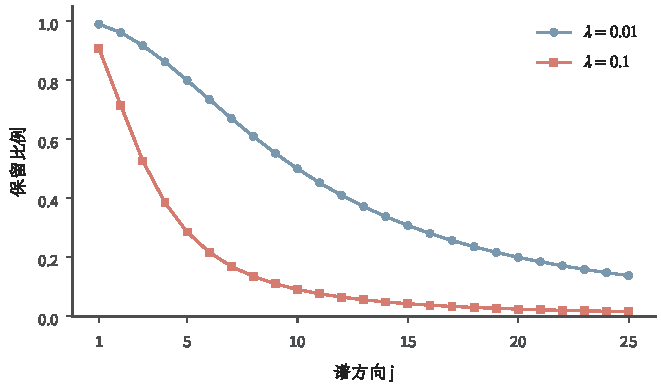
\includegraphics[width=\linewidth]{figures/math-preparation/analysis-geometry/functional-spectral-shrinkage.pdf}
 \caption{教学谱$\mu_j=j^{-2}$上的收缩比例$\mu_j/(\mu_j+\lambda)$。蓝、红线使用$\lambda=0.01$和$0.1$，点标出前$25$个方向；增大正则化后更多方向被抑制。有效维度的定义仍对全部谱方向求和。}
 \label{fig:functional-spectral-shrinkage}
\end{figure}

矩阵迹汇总有限个方向的贡献；无限维空间中的方向可能有无穷多个，因此还要核对这份
总量是否有限。下面把算子条件与所选正则化尺度分开。
\begin{definition}[迹类条件与有效维度]
\label{def:functional-trace-effective-dimension}
设$A$为Hilbert空间上的紧线性算子。$A^*A$的正特征值开方后得到奇异值$s_j(A)$，
按重数排列；若只有有限个，可在其后补零。若$\sum_j s_j(A)<\infty$，称$A$为
\term{迹类算子}（trace-class operator）。对正算子，这等价于非负特征值之和有限，
它的迹就是这个和。

若紧正算子$T_K$的正特征值为$(\mu_j)$，给定$\lambda>0$，其
\term{有效维度}（effective dimension）定义为
\begin{equation}
  d_{\mathrm{eff}}(\lambda)
  =
  \sum_{j\geq1}\frac{\mu_j}{\mu_j+\lambda}
  \label{eq:functional-effective-dimension}
\end{equation}
这里要求右侧级数有限；等价地，
\[
  d_{\mathrm{eff}}(\lambda)
  =
  \operatorname{tr}\bigl(T_K(T_K+\lambda I)^{-1}\bigr)
\]
并要求$T_K(T_K+\lambda I)^{-1}$为迹类。
\end{definition}
迹类要求有限的谱总量，有效维度则先按尺度收缩各方向，再汇总它们的贡献。
在上述Mercer条件下，$\sum_j\mu_j<\infty$，所以
$d_{\mathrm{eff}}(\lambda)\leq\lambda^{-1}\sum_j\mu_j<\infty$。
每个谱方向按其相对于
$\lambda$的大小贡献$0$到$1$之间的量。$\mu_j\gg\lambda$的方向近似贡献$1$，
$\mu_j\ll\lambda$的方向贡献很小。有限样本Gram矩阵也有对应量
\[
  \operatorname{tr}\left(
    \bm{K}(\bm{K}+n\lambda\bm{I}_n)^{-1}
  \right),
\]
但它依赖当前输入与归一化约定，不应和总体积分算子的
$d_{\mathrm{eff}}(\lambda)$混为同一数值。

有效维度不是代数维数。无限维空间在固定$\lambda$下可以有有限有效维度；反过来，一个
有限参数化若参数到函数的映射高度敏感，也可能形成很大的函数集合。参数数量、谱衰减、
导数规则性和范数半径从不同方面描述复杂度。后续核正则化会同时使用谱和范数；神经切线核
只在相应线性化条件下提供这种空间解释，深层网络本身的复杂度不能无条件等同于某个固定核
的有效维度。

\section{逼近能力与表示选择}
\label{sec:functional-approximation-capacity-representation}

\subsection{稠密性与一致逼近}

沿用定义~\ref{def:functional-density}的稠密性，下面不再只判断极限是否存在，
而是寻找能随目标与精度构造出的具体表示。稠密性是一项表示存在性结论：它允许逼近器依赖目标和精度，却
没有说明需要多少参数、怎样找到逼近器，或从有限观测能否识别它。

多项式提供一个基本例子。对$f\in C([0,1])$，定义Bernstein多项式
\begin{equation}
  (B_mf)(x)
  =
  \sum_{j=0}^{m}
  f\left(\frac{j}{m}\right)
  \binom{m}{j}x^j(1-x)^{m-j}.
  \label{eq:functional-bernstein-polynomial}
\end{equation}
权重非负且由二项式定理知其和为$1$，所以$B_mf(x)$是邻近网格函数值的加权平均。

\begin{theorem}[Bernstein逼近定理]
\label{thm:functional-weierstrass-bernstein}
对每个$f\in C([0,1])$，
\[
  \lVert B_mf-f\rVert_{\infty}\longrightarrow0.
\]
因此，多项式在$C([0,1])$的一致范数下稠密。
\end{theorem}

\begin{proof}
连续函数在紧区间上一致连续且有界。记
$M=\lVert f\rVert_{\infty}$。给定$\varepsilon>0$，可取$\delta>0$使
$|u-x|<\delta$时$|f(u)-f(x)|<\varepsilon/2$。

对固定$x$，把式\eqref{eq:functional-bernstein-polynomial}中的权重记为
$w_{m,j}(x)$。除$\sum_jw_{m,j}(x)=1$外，直接对二项式求导可得
\[
  \sum_{j=0}^{m}
  \left(\frac{j}{m}-x\right)^2w_{m,j}(x)
  =
  \frac{x(1-x)}{m}
  \leq\frac{1}{4m}.
\]
将网格点分为
$|j/m-x|<\delta$与$|j/m-x|\geq\delta$两组。近处一组的函数值差小于
$\varepsilon/2$。远处一组的总权重满足
\[
  \sum_{|j/m-x|\geq\delta}w_{m,j}(x)
  \leq
  \frac{1}{\delta^2}
  \sum_{j=0}^{m}
  \left(\frac{j}{m}-x\right)^2w_{m,j}(x)
  \leq\frac{1}{4m\delta^2}.
\]
因此对所有$x\in[0,1]$，
\[
  |B_mf(x)-f(x)|
  \leq
  \frac{\varepsilon}{2}
  +
  2M\frac{1}{4m\delta^2}.
\]
取$m$足够大使第二项不超过$\varepsilon/2$，便得到一致误差不超过
$\varepsilon$。界对所有$x$使用同一个$m$，所以结论是一致收敛。
\end{proof}

证明展示了规则性怎样影响逼近：目标的一致连续性控制近处网格值的变化，二项式权重的二阶
离散矩控制远处权重。如果已知更强的光滑性，可以得到更具体的误差速率；只有连续性时，
定理仍给出存在性，但不承诺对所有连续函数共享一个与目标无关的快速速率。

多项式同时调整全域系数，分段线性样条则把改动限制在少数相邻区间。设
$a=x_0<x_1<\cdots<x_m=b$，最大网格宽度为
$h=\max_j(x_{j+1}-x_j)$，并令$S_hf$在结点处等于$f$、在每个小区间上线性插值。
若$\omega_f(h)=\sup_{|x-z|\leq h}|f(x)-f(z)|$是$f$的连续模，则
\[
  \lVert f-S_hf\rVert_\infty\leq\omega_f(h).
\]
这是因为区间内的插值值是两个端点函数值的凸组合，每个端点距当前点都不超过$h$。
当$f$二阶连续可微时，Taylor余项进一步给出
\[
  \lVert f-S_hf\rVert_\infty
  \leq
  \frac{h^2}{8}\lVert f''\rVert_\infty.
\]
前一个界只依赖连续性，后一个界用更强规则性换取二阶误差。在固定结点位置时，改变一个样条结点的函数值只改变相邻
片段，而改变一个全局多项式系数通常会影响整个区间；这是局部表示与全局表示的结构差别，
不是两种误差范数之间的优劣结论。
为看清“一个局部改动”的范围，图~\ref{fig:functional-basis-locality}固定同一个中心，
只增加一个单位系数。样条帽函数在相邻结点外严格为零；Bernstein基在整个开区间内非零；
高斯基虽快速衰减，仍在所有位置非零。局部性需要由基函数的支撑或衰减式判断，不能由参数个数判断。
\begin{figure}[htbp]
 \centering
 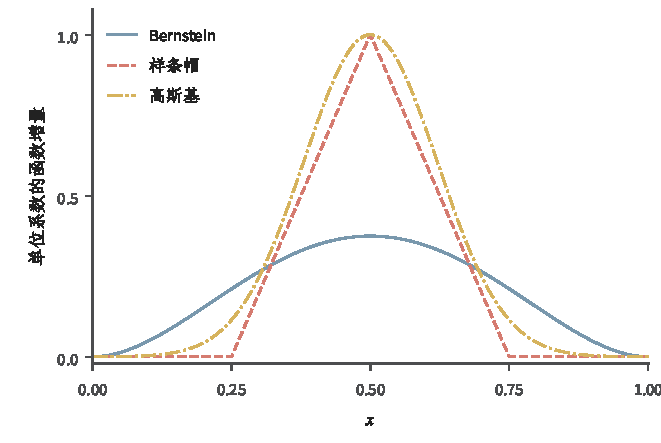
\includegraphics[width=\linewidth]{figures/math-preparation/reader-revision-analysis/functional-basis-locality.pdf}
 \caption{单个系数改变对函数的影响。蓝线为$6x^2(1-x)^2$，即四阶Bernstein多项式的中心基；
 红线为中心$1/2$、相邻结点$1/4,3/4$的线性样条帽；黄线为中心$1/2$、宽度$0.12$的高斯基。
 系数增量均为$1$，不另行缩放峰高；图比较作用范围，未比较三种方法的最优逼近误差。}
 \label{fig:functional-basis-locality}
\end{figure}


\subsection{多项式、样条、核展开与神经网络}

固定目标
\[
  f_\star(x)=\left|x-\frac12\right|,
  \qquad x\in[0,1],
\]
可以看清表示选择的差异。全局多项式用一组遍及整个区间的基函数逼近折点；分段线性样条
只需把$1/2$设为结点，就能精确表示$f_\star$。使用宽度$\sigma>0$的高斯核
\[
  K_\sigma(x,z)
  =
  \exp\left(-\frac{(x-z)^2}{2\sigma^2}\right)
\]
时，可以由若干主要作用于中心附近的核截面$K_\sigma(\,\cdot\,,x_i)$组合出平滑逼近。
高斯核离开中心后衰减，却没有紧支撑；“局部”不表示中心以外恰好为零。有限组合仍是
光滑函数，不能在有限核宽度下精确产生折点。带ReLU激活的单隐藏层网络则可直接写成
\[
  f_\star(x)
  =
  \operatorname{ReLU}\left(x-\frac12\right)
  +
  \operatorname{ReLU}\left(\frac12-x\right).
\]
这些差别来自表示与目标规则性的匹配，不能只由“哪一类更通用”判断。

\begin{table*}[htbp]
 \centering\small
 \begin{tabularx}{\linewidth}{@{}lXX@{}}
 \toprule
 表示 & 对$f_\star(x)=|x-1/2|$的有限表示 & 调整的范围\\
 \midrule
 全局多项式 & 可逼近，有限次数不能精确产生折点 & 一个系数通常影响整个区间\\
 分段线性样条 & 将$1/2$设为结点即可精确表示 & 结点邻域内的分段变化\\
 固定正宽度的高斯核有限和 & 保持光滑，可逼近但不能精确产生折点 & 核中心附近的变化，宽度决定影响范围\\
 两个ReLU单元 & 上式直接给出精确表示 & 隐藏单元的位置和方向决定折点\\
 \bottomrule
 \end{tabularx}
 \caption{同一个连续目标的不同表示。有限表示的结构与整个表示族的稠密性是不同问题。}
 \label{tab:functional-representation-comparison}
\end{table*}

网络表示的逼近能力也需要写清激活条件。仅仅“含非线性”还不够：若
$\sigma(t)=t^2$，所有单隐层有限和仍是次数至多为$2$的多项式，无论增加多少单元都不能
得到任意高次目标。下面的结论允许增加宽度，并要求隐藏单元具有偏置。

\begin{theorem}[单隐藏层的通用逼近]
\label{thm:functional-universal-approximation}
设$\mathcal X\subseteq\mathbb R^d$为非空紧集，$f:\mathcal X\to\mathbb R$连续，
$\sigma:\mathbb R\to\mathbb R$连续且不是多项式。对任意$\varepsilon>0$，存在有限
宽度$m$、实数$a_j,b_j,c$以及$\bm w_j\in\mathbb R^d$，使
\begin{equation}
 \begin{aligned}
 g(\bm x)&=c+\sum_{j=1}^m a_j\sigma(\bm w_j^{\top}\bm x+b_j),\\
 \sup_{\bm x\in\mathcal X}|g(\bm x)-f(\bm x)|&<\varepsilon.
 \end{aligned}
 \label{eq:functional-universal-approximation}
\end{equation}
\end{theorem}

这是Leshno等结果在连续激活情形下的表述\scite{leshno1993approximation}
Sigmoid、Tanh与ReLU都满足激活条件；定理不要求处处可微。连续S形激活在两端分别趋于
$0$与$1$，是非多项式条件的一个常见特例。特别地，紧立方体上的有限和
\begin{equation}
 g(\bm x)=\sum_{j=1}^m a_j\sigma(\bm w_j^{\top}\bm x+b_j)
 \label{eq:functional-sigmoidal-network}
\end{equation}
已能一致逼近连续目标。定理证明涉及更一般的函数空间分离与激活的非多项式性质；本章
前面的Bernstein证明提供稠密性的完整构造，折线与ReLU的对应则给出一维网络版本的直接
构造直觉。

宽度$m$是在给定$f$和$\varepsilon$之后选择的。存在某个表示不保证固定宽度足够，
也不保证训练算法找到参数、有限样本足够或紧集之外的外推准确。向量值目标可以逐坐标
使用结论，再合并有限个单元；目标含跳跃时则不能套用连续目标的一致逼近结论。

不同激活与误差空间还有其他普适逼近版本，但每个版本都必须重新写清定义域、目标集合和
激活条件。它们共同的量词形式是
\[
  \forall f\ \forall\varepsilon>0\
  \exists\text{网络规模与参数，使误差小于 }\varepsilon.
\]
这个陈述没有给出以下任何一项无条件保证：所需网络很小，参数能由可承受的计算找到，
训练算法会到达该参数，或者有限样本上的拟合会在新输入上保持准确。多项式的稠密性也有
同样边界。表示存在、参数规模、优化可计算性和统计泛化是四个不同问题。

误差范数同样决定结论。若只要求$L^2$误差小，逼近器可以在小测度区域出现较大尖峰；若
要求一致误差小，则必须同时控制所有输入。若目标定义在非紧域上，还需要指定加权范数、
局部一致收敛或尾部条件。若目标含不连续点，连续逼近器不可能在整个定义域上一致收敛到
目标，却仍可能在$L^p$意义下逼近。讨论“普适”时必须同时写清目标集合、定义域、逼近器
的并集和误差度量。

\section{函数类的方向、幅度与规则性}
\label{sec:functional-class-size-smoothness}

\subsection{范数球与函数幅度}

上一节允许表示规模随精度增加；这保证可以接近目标，却没有限制候选族还能出现哪些变化。
本节分别限制幅度、导数的累计变化，以及双变量关系中可用的方向数。稠密的表示族可能非常大。若允许多项式次数和系数任意增长，它既能逼近平滑趋势，也能产生
快速振荡。实际分析通常固定一个半径$B$，考察范数球
\[
  \mathcal{F}_B
  =
  \{f\in\mathcal{V}:\lVert f\rVert_{\mathcal{V}}\leq B\}.
\]
半径限制只有结合范数含义才有信息。$L^2$范数限制函数整体能量，却不直接限制导数；
下一小节会先把导数定义为积分意义下的对象，再用Sobolev范数同时限制函数值与直到某个
非负整数阶的导数，因而抑制快速振荡。Lipschitz约束
$|f(x)-f(z)|\leq L|x-z|$则直接限制输入变化造成的输出变化。它们控制的对象不同，
不能由一个较小的参数数量替代。

在RKHS中，式\eqref{eq:functional-rkhs-pointwise-bound}说明核对角有界时，核范数球
统一控制点值。两个输入之间还有
\begin{equation}
  |f(x)-f(z)|
  \leq
  \lVert f\rVert_{\mathcal{H}_K}
  \lVert K_x-K_z\rVert_{\mathcal{H}_K},
  \label{eq:functional-rkhs-modulus-bound}
\end{equation}
而
\[
  \lVert K_x-K_z\rVert_{\mathcal{H}_K}^2
  =
  K(x,x)+K(z,z)-2K(x,z).
\]
因此，核既确定可用方向，也确定输入变化在空间中有多远；半径再限制沿这些方向的幅度。
改变核与改变正则化强度不是同一操作。

\subsection{弱导数与Sobolev空间}

经典导数要求逐点极限存在，会排除带尖点但整体仍然规则的函数。为了只保留积分运算真正
需要的变化信息，可以反过来要求分部积分恒等式成立：让导数先作用在光滑测试函数上，
再检验能否由另一个普通函数表示结果。测试函数用来探测局部变化，其紧支撑意味着它在
靠近区域边界处恒为零，因此不会引入边界项。
\begin{definition}[测试函数与局部可积性]
\label{def:functional-tests-local-integrability}
设$U\subseteq\mathbb R^d$开。函数$\varphi$的支撑是集合
$\{\bm x\in U:\varphi(\bm x)\neq0\}$在$\mathbb R^d$中的闭包。
$C_c^\infty(U)$由无限次连续可微、支撑为$U$内紧集的实函数组成。
空间$L^1_{\mathrm{loc}}(U)$由对每个紧集$K\subset U$满足
$\int_K|f|<\infty$的可测函数的几乎处处等价类组成。
\end{definition}
前一项让测试远离边界，后一项让与任何局部测试函数的积分有限；不要求$f$在整个$U$上可积。
\begin{definition}[弱导数]
\label{def:functional-weak-derivative}
设$U\subseteq\mathbb R^d$开，$f\in L^1_{\mathrm{loc}}(U)$。
取多重指标$\alpha=(\alpha_1,\ldots,\alpha_d)\in\mathbb{N}_0^d$，记
$|\alpha|=\sum_{j=1}^d\alpha_j$，
$D^\alpha=\partial_1^{\alpha_1}\cdots\partial_d^{\alpha_d}$。若存在
$g_\alpha\in L^1_{\mathrm{loc}}(U)$使每个
$\varphi\in C_c^\infty(U)$都满足
\begin{equation}
  \int_U f(\bm{x})D^\alpha\varphi(\bm{x})\,\mathrm{d}\bm{x}
  =
  (-1)^{|\alpha|}
  \int_U g_\alpha(\bm{x})\varphi(\bm{x})\,\mathrm{d}\bm{x},
  \label{eq:functional-weak-derivative}
\end{equation}
就称$g_\alpha$为$f$的$\alpha$阶\term{弱导数}（weak derivative），记为
$D^\alpha f$，按几乎处处等价理解。
\end{definition}
式\eqref{eq:functional-weak-derivative}把经典分部积分当作定义；
测试函数的紧支撑使边界项消失，因此这个定义本身不需要给$U$另加边界条件。

有了弱导数，就可以同时累计函数值与导数的平方误差，得到比$L^2$更强的规则性要求。
\begin{definition}[整数阶平方可积Sobolev空间]
\label{def:functional-sobolev-space}
设$U\subseteq\mathbb R^d$为开集，$m\in\mathbb N_0$。Sobolev空间
\[
  W^{m,2}(U)
  =
  \left\{
    f\in L^2(U):
    D^\alpha f\in L^2(U),\ |\alpha|\leq m
  \right\}
\]
配备范数
\begin{equation}
  \lVert f\rVert_{W^{m,2}(U)}^2
  =
  \sum_{|\alpha|\leq m}
  \lVert D^\alpha f\rVert_{L^2(U)}^2.
  \label{eq:functional-sobolev-norm}
\end{equation}
其中$D^0f=f$，所有导数均按弱导数理解，元素按几乎处处等价识别。
\end{definition}
当$U=(a,b)$为一维区间时，$W^{m,2}(a,b)$也常记作$H^m(a,b)$，式
\eqref{eq:functional-sobolev-norm}相应写成
\[
  \lVert f\rVert_{H^m(a,b)}^2
  =
  \sum_{r=0}^{m}
  \int_a^b|D^r f(x)|^2\,\mathrm{d}x.
\]
这里$m\in\mathbb{N}_0$，各阶导数都按上面的弱导数定义理解；非整数阶Sobolev空间需要
其他定义，不由这个有限求和给出。
例如一维函数$f(x)=|x|$在原点没有经典导数，但其一阶弱导数几乎处处等于
$\operatorname{sign}(x)$；在有界区间上，它仍属于$W^{1,2}$。尖点因而不会自动排除
积分意义下的平滑性。

在$(-1,1)$上把积分分成左右两段，可以直接核对这一弱导数：
\[
 \int_{-1}^1 |x|\varphi'(x)\,\mathrm dx
 =\int_{-1}^0\varphi(x)\,\mathrm dx-\int_0^1\varphi(x)\,\mathrm dx
 =-\int_{-1}^1\operatorname{sign}(x)\varphi(x)\,\mathrm dx.
\]
两侧在$0$处的边界项都为零，原点处任意指定的单个导数值也不会改变积分。
图~\ref{fig:functional-weak-derivative}将这两条函数并列：弱导数允许用一个几乎处处
确定的函数保存变化信息，而不要求补出尖点处不存在的经典导数。
\begin{figure*}[htbp]
 \centering
 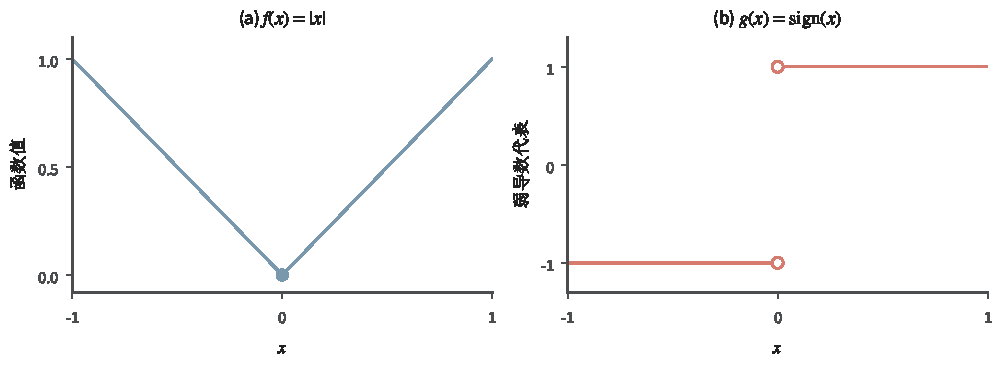
\includegraphics[width=\linewidth]{figures/math-preparation/concept-revision-analysis-functional/weak-derivative.pdf}
 \caption{$f(x)=|x|$与其一阶弱导数$g(x)=\operatorname{sign}(x)$。左图原点为连续尖点；右图两段分别为$-1$与$1$，空心端点表示经典导数在原点未定义。弱导数在原点的代表值可以任取，积分恒等式不受影响。}
 \label{fig:functional-weak-derivative}
\end{figure*}

几乎处处存在经典导数仍不足以保证该导数就是弱导数。阶跃函数
$h(x)=\mathbb I\{x>0\}$几乎处处的经典导数为零，但
$\int_{-1}^1h\varphi'=-\varphi(0)$一般不为零。若能由某个局部可积函数$g$表示
它的弱导数，取支撑逐渐缩到原点、满足$0\leq\varphi_n\leq1$且$\varphi_n(0)=1$的
光滑测试函数，则$|\int g\varphi_n|\to0$，却应等于$1$，矛盾。因此跳跃与连续尖点
在弱导数意义下也有不同表现；单凭“只在一个点不可微”无法判断Sobolev成员资格。

$W^{m,2}(U)$是Hilbert空间。证明完备性时，取其中的柯西列$(f_n)$。对每个
$|\alpha|\leq m$，序列$(D^\alpha f_n)$在$L^2(U)$中都是柯西列，故收敛到某个
$g_\alpha\in L^2(U)$，其中$g_0$记为$f$。把$f_n$的弱导数恒等式分别在两侧取极限；
Cauchy--Schwarz不等式保证与固定测试函数的积分连续，于是
\[
  \int_U fD^\alpha\varphi
  =
  (-1)^{|\alpha|}\int_U g_\alpha\varphi.
\]
因此$g_\alpha=D^\alpha f$，并且$f_n\to f$于
$W^{m,2}(U)$。若另外要求零边界值或其他边界条件，还须证明满足该条件的子空间闭；
一般Sobolev空间的完备性不能替这些边界条件作保证。

\subsection{函数的低秩分解}

前面的表示用基函数、核截面或非线性单元描述一个输入函数。若输入本身分成两组，
还可以利用两组变量之间有限个可分离方向来压缩表示；这就是函数低秩结构的问题。
矩阵的秩在此取本科线性代数中的含义，其系统讨论见第~\ref{chap:linear-algebra}章。
设$p\in\mathcal{P}$表示一种预测或模型索引，
$q\in\mathcal{Q}$表示一种查询、条件或检验索引，量
$E(p,q)\in\mathbb{R}$记录二者组合后的函数值或误差。选取有限对象
$p_1,\ldots,p_m$与$q_1,\ldots,q_n$，可组成矩阵
\[
  \bm{E}_{i,j}=E(p_i,q_j).
\]
若存在映射$\bm{u}:\mathcal{P}\to\mathbb{R}^r$与
$\bm{v}:\mathcal{Q}\to\mathbb{R}^r$使
\begin{equation}
  E(p,q)
  =
  \langle\bm{u}(p),\bm{v}(q)\rangle,
  \label{eq:functional-bilinear-factorization}
\end{equation}
则任意有限矩阵$\bm{E}$的秩至多为$r$。低秩的含义是所有双索引变化都可由$r$个潜在
方向组合，而不是矩阵元素数目少。

Cauchy--Schwarz不等式还把因子尺度传到每个矩阵元素：
\[
  |E(p,q)|
  \leq
  \lVert\bm{u}(p)\rVert_2
  \lVert\bm{v}(q)\rVert_2.
\]
所以秩控制可用方向数，因子范数控制沿这些方向能够产生的幅度。

秩本身只计方向数，不控制数值尺度。若把因子同时变换为
$\bm{u}'(p)=c\bm{u}(p)$和
$\bm{v}'(q)=\bm{v}(q)/c$，式
\eqref{eq:functional-bilinear-factorization}不变，单边因子范数却可以任意改变。
因此，用低秩结构控制误差或计算时，通常还要固定
\[
  \sup_{p\in\mathcal{P}}\lVert\bm{u}(p)\rVert_2\leq B_u,
  \qquad
  \sup_{q\in\mathcal{Q}}\lVert\bm{v}(q)\rVert_2\leq B_v,
\]
或采用对这种缩放更稳定的矩阵范数。方向数$r$与幅度$B_uB_v$承担不同作用。

严格低秩也可能过强。若存在
\[
  E(p,q)
  =
  \langle\bm{u}(p),\bm{v}(q)\rangle+\eta(p,q),
  \qquad
  \sup_{p,q}|\eta(p,q)|\leq\delta,
\]
则$r$描述结构化主项的方向数，$\delta$描述剩余表示误差。增大$r$可能减小$\delta$，
但不会自动给出怎样找到因子、怎样选择查询或怎样由有限观测估计矩阵。代数上的低秩、
因子范数、逼近误差、数据访问条件和计算过程仍须分别说明。

强化学习中的某些复杂度概念会把模型与分布之间的Bellman残差组织成类似矩阵，再研究其
秩或因子化结构。那里的矩阵条目、可实现性、查询协议和样本保证依赖具体决策对象，必须在
相应章节重新定义。仅仅看到某个双线性表达，既不能直接称其为Bellman秩，也不能推出高效
学习。本节提供的是识别这类结构时所需的共同语言。

\section{函数类的覆盖数与度量熵}
\label{sec:functional-combinatorial-metric-complexity}

\subsection{组合模式与距离近似}

第~\ref{chap:combinatorics}章的第~\ref{sec:comb-families-counting}节已经建立
打散、生长函数与组合维度：它们考察有限输入上能独立实现哪些输出选择。本节转向
函数近似，问在指定误差范围内，需要多少个代表函数才能近似整个函数类。
模式是否可实现与近似误差有多大，是两个需要分别说明的问题。

对非空输入空间$\mathcal X$上的非空二值函数类$\mathcal F\subseteq\{0,1\}^{\mathcal X}$及输入组$S=(x_1,\ldots,x_n)$，
沿用组合章的限制类记号和定义~\ref{def:growth-function}：
\begin{equation}
 \mathcal F|_S=\{(f(x_1),\ldots,f(x_n)):f\in\mathcal F\},
 \qquad \Pi_{\mathcal F}(n)\text{表示该类的生长函数}.
 \label{eq:functional-growth-function}
\end{equation}
固定$S$只观察这组输入，生长函数还要在所有$n$个输入的选择之间取最坏情况。
定义~\ref{def:vc-dimension}与引理~\ref{lem:sauer-shelah}提供模式数的组合控制，
但没有为两个函数在整个定义域上的误差选择距离。

例如实线上由$a\in\mathbb R$索引的阈值函数类，
$f_a(x)=\mathbb{I}\{x\geq a\}$，在$n$个互异且有序的输入上只能产生$n+1$种模式，
而全部二值函数可以产生$2^n$种模式。但只要$a\neq b$，就有
$\sup_{x\in\mathbb R}|f_a(x)-f_b(x)|=1$：两个阈值之间总有输入使输出不同。
在固定$n$个输入上模式有限，并不说明另一个阈值函数能在所有输入上提供小于$1$的
最坏误差。前一种比较统计输出模式，后一种比较函数在指定位置上的差值。

有限函数类给出另一个直接的上界。若$\#\mathcal{F}=M<\infty$，每个函数在固定输入组上
至多贡献一种模式，因而
\[
  \Pi_{\mathcal{F}}(n)\leq\min\{M,2^n\}.
\]
例如只含两个常值函数$f_0(x)=0$与$f_1(x)=1$的函数类，在任意非空输入组上恰好产生
全零和全一两种模式，所以$\Pi_{\mathcal{F}}(n)=2$对所有$n\geq1$成立。有限类的函数数目
限制了模式总数，但不同函数在某组输入上可能给出相同限制，因此一般只能得到上界。

实值函数的伪维与胖打散维同样回用组合章第~\ref{sec:comb-real-valued-threshold-margins}节。
伪维检查能否跨过固定阈值，胖打散维还规定阈值两侧的间隔。函数近似则需要另行规定
比较哪些输入、怎样汇总误差：上确界误差关注最坏位置，平方积分误差关注测度加权的
整体差异。选定这种距离后，才能用代表函数的数量描述给定精度下的近似规模。

\subsection{覆盖数与度量熵}

把候选函数逐个列出可能需要无穷多个对象。如果容许误差不超过$\varepsilon$，一组有限
代表却可能已经够用。覆盖数记录的是这组代表至少需要多少个，而不是原类有多少个函数。
\begin{definition}[函数类的覆盖数与度量熵]
\label{def:functional-covering-number}
设$\mathcal F$为非空函数类，$d$为定义~\ref{def:analysis-pseudometric}中的伪距离；
只看有限输入时，两个不同函数的样本距离可能为零。给定正半径$\varepsilon>0$，
若有限集合$\mathcal{C}\subseteq\mathcal{F}$满足：对每个$f\in\mathcal{F}$，存在
$g\in\mathcal{C}$使$d(f,g)\leq\varepsilon$，则$\mathcal{C}$称为
$\varepsilon$-覆盖。最小覆盖大小记为
\[
  N(\varepsilon,\mathcal{F},d),
\]
若不存在有限$\varepsilon$-覆盖，约定$N=+\infty$；其对数称为度量熵。零半径的覆盖也沿用上述约定，
用于下文$L=0$时的复合函数类。覆盖数回答的是：在指定误差尺度下，需要多少个代表函数才能近似整个
函数类。
\end{definition}
无穷函数类在正尺度下仍可能有有限覆盖；缩小容许误差时，覆盖数只能不减。
覆盖球可以互相重叠，也可以伸到函数类之外，但这里的球心必须属于$\mathcal F$。

距离的选择会改变覆盖对象。常见的$d_\infty$用于有界实函数类，
$d_{L^2(\mu)}$用于同一测度$\mu$下的平方可积函数类，而样本距离$d_S$取非空
输入组$S=(x_1,\ldots,x_n)$、$n\geq1$；这些条件保证下列距离有限：
\begin{align*}
  d_{\infty}(f,g)
  &=
  \sup_{x\in\mathcal{X}}|f(x)-g(x)|,\\
  d_{L^2(\mu)}(f,g)
  &=
  \left(
    \int_{\mathcal{X}}|f(x)-g(x)|^2\,\mathrm{d}\mu(x)
  \right)^{1/2},\\
  d_S(f,g)
  &=
  \left(
    \frac1n\sum_{i=1}^{n}|f(x_i)-g(x_i)|^2
  \right)^{1/2}.
\end{align*}
$d_\infty$同时控制所有输入，$d_{L^2(\mu)}$只控制测度$\mu$加权的整体差异，$d_S$
只看给定有限输入。一个样本距离下很小的覆盖未必控制样本外的函数差异；一个
$L^2(\mu)$覆盖也未必控制$\mu$几乎不赋质量的区域。后续概率论章建立随机样本后，
才会讨论怎样把这些确定性覆盖结构接到同时误差概率界。

有限输入上的量化给出一个可以直接核对的覆盖。给定$\varepsilon>0$，设每个$f\in\mathcal{F}$在
$S=(x_1,\ldots,x_n)$上都取值于$[-B,B]$。把该区间分成长度不超过
$\varepsilon$的小区间，并对每个被$\mathcal{F}|_S$占据的$n$维网格单元选取一个
代表函数。落在同一单元的两个函数在每个$x_i$处相差不超过$\varepsilon$，因而其
$d_S$距离也不超过$\varepsilon$。由此得到
\[
  N(\varepsilon,\mathcal{F},d_S)
  \leq
  \left(1+\left\lceil\frac{2B}{\varepsilon}\right\rceil\right)^n.
\]
这个界同时写出了值域$[-B,B]$、分辨率$\varepsilon$和输入数$n$。它只覆盖
$S$上可见的取值向量，不控制其他输入，也不声称该上界达到最小覆盖大小。

图~\ref{fig:functional-covering-centers}把量化的含义放到一个可精确计算的函数族中。
令$f_{a,b}(x)=a+bx$，$a,b\in[-1,1]$，并取$S=(-1,1)$，则
\[
 d_S(f_{a,b},f_{a',b'})^2
 =\tfrac12\bigl((\Delta a-\Delta b)^2+(\Delta a+\Delta b)^2\bigr)
 =(\Delta a)^2+(\Delta b)^2.
\]
因此样本距离恰是系数平面中的欧氏距离。把每个坐标分成三个等宽区间，取九个格心，
就得到半径$\sqrt2/3$的覆盖：任意函数与其格心代表的两项系数差均不超过$1/3$。
这证明$N(\sqrt2/3,\mathcal F,d_S)\leq9$，没有证明九个是最少数量。
\begin{figure}[htbp]
 \centering
 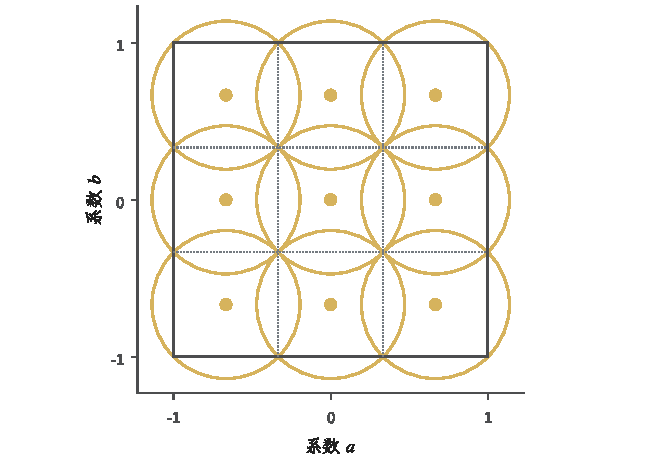
\includegraphics[width=\linewidth]{figures/math-preparation/concept-revision-analysis-functional/covering-centers.pdf}
 \caption{仿射函数族的有限覆盖。方形表示$a,b\in[-1,1]$，九个实心点是类内代表，圆的半径为$\sqrt2/3$。每个小方格都被对应格心的闭球覆盖；圆的重叠与越出方形的部分均不影响覆盖要求。}
 \label{fig:functional-covering-centers}
\end{figure}

覆盖结构还可以由函数类运算传播。若$\mathcal{F}$与$\mathcal{G}$在同一上确界距离下
分别有$\varepsilon_F$与$\varepsilon_G$覆盖，则
\[
  \mathcal{F}+\mathcal{G}
  =
  \{f+g:f\in\mathcal{F},\ g\in\mathcal{G}\}
\]
有半径$\varepsilon_F+\varepsilon_G$、大小至多为两个覆盖大小乘积的覆盖。若
$\varphi:\mathbb{R}\to\mathbb{R}$是$L$-Lipschitz函数，则把
$\mathcal{F}$的$\varepsilon$-覆盖逐点送入$\varphi$，得到
$\varphi\circ\mathcal{F}$的$L\varepsilon$-覆盖。这些关系说明组合结构怎样累积
复杂度，却不自动给出有限样本泛化结论。

覆盖数随距离与误差半径改变，组合维度则随输出区分规则改变。二者都需要明确函数类
与输入对象；把计数界或覆盖界用于学习保证时，还要另加抽样和概率条件。

\section{自适应输入上的函数类复杂度}
\label{sec:functional-sequential-classes-low-rank}

\subsection{查询树与序贯复杂度}

前一节把输入$x_1,\ldots,x_n$预先固定。序贯问题允许第$t$个输入根据此前反馈变化，
单个输入序列因而不能列出所有可能路径。这里用二叉树表达分支，并以
$\epsilon_t\in\{-1,1\}$标记第$t$步选择的分支；$\epsilon_t$只是抽象路径标签，不必
等于实值函数输出$f(\bm{x}_t)$。若具体问题的反馈不是二元值，还需另行给出编码规则或
改用相应的分支集合。
\begin{definition}[二叉查询树]
\label{def:functional-query-tree}
设$\mathcal X$为非空输入集合，$T\geq1$为整数。深度为$T$的\term{查询树}（query tree）由映射
\[
  \bm{x}_t:\{-1,1\}^{t-1}\to\mathcal{X},
  \qquad t=1,\ldots,T,
\]
组成。这里$\{-1,1\}^0$只有空路径，根节点因而是一个固定输入$\bm{x}_1$；在路径
$\bm{\epsilon}=(\epsilon_1,\ldots,\epsilon_T)$上，第$t$步访问
$\bm{x}_t(\epsilon_1,\ldots,\epsilon_{t-1})$。同一个函数$f$沿该路径产生
\[
  \bigl(
    f(\bm{x}_1),
    f(\bm{x}_2(\epsilon_1)),
    \ldots,
    f(\bm{x}_T(\epsilon_1,\ldots,\epsilon_{T-1}))
  \bigr).
\]
\end{definition}
树同时编码所有按过去分支的输入选择规则，本身没有给路径指定概率。

图~\ref{fig:functional-query-tree}只展开两层，便能看见这一信息约束：查询$x_0$之后，
下一次查询取$x_-$还是$x_+$由已出现的分支决定。覆盖中心必须提前为两个可能的下一步
都指定值，不能在分支确定后临时增加一棵新的中心树。
\begin{figure}[htbp]
 \centering
 % Simple three-query tree; centers assign values before a branch is selected.
\begin{tikzpicture}[figure picture,x=1mm,y=1mm,font=\figurefont\footnotesize,
  query/.style={draw=FigureStroke,line width=1pt,rounded corners=1.2mm,
    minimum width=24mm,minimum height=10mm,fill=white,align=center},
  branch/.style={-{Stealth[length=2.2mm,width=1.4mm]},draw=FigureStroke,
    line width=1.1pt,rounded corners=1.2mm}]
 \node[query] (root) at (0,0) {$x_0$};
 \node[query] (left) at (-27,-28) {$x_-$};
 \node[query] (right) at (27,-28) {$x_+$};
 \draw[draw=FigureStroke,line width=1.1pt] (root.south) -- (0,-12);
 \draw[branch] (0,-12) -| (left.north);
 \draw[branch] (0,-12) -| (right.north);
 \node[above,font=\figurefont\footnotesize] at (-16,-12) {$\epsilon_1=-1$};
 \node[above,font=\figurefont\footnotesize] at (16,-12) {$\epsilon_1=+1$};
 \node[right,font=\figurefont\footnotesize,text=FigureInk] at (14,0) {$v_1$};
 \node[below,font=\figurefont\footnotesize,text=FigureInk] at (-27,-35) {$v_2(-1)$};
 \node[below,font=\figurefont\footnotesize,text=FigureInk] at (27,-35) {$v_2(+1)$};
\end{tikzpicture}

 \caption{深度为$2$的固定查询树。根查询$x_0$，左右分支对应$\epsilon_1=-1$与$+1$；下方的$v_1,v_2(\pm1)$是一棵覆盖中心在三个节点预先指定的值，表示近似值而非真实反馈。固定两点输入只观察其中一条路径。}
 \label{fig:functional-query-tree}
\end{figure}

在固定输入上，覆盖中心是一组函数值；在查询树上，它必须为每个可能访问的节点预先
指定一个实数。下面的覆盖条件沿每条路径比较误差，中心集合仍在路径出现之前确定。
\begin{definition}[序贯覆盖与序贯覆盖数]
\label{def:functional-sequential-cover}
给定深度为$T$的查询树$\bm x$、非空实值函数类$\mathcal F$和$\varepsilon>0$。
实数树$v=(v_t)$的每层映射为$v_t:\{-1,1\}^{t-1}\to\mathbb R$。若这些树组成的
有限集合$\mathcal C$满足：对每个$f\in\mathcal F$和每条路径$\bm\epsilon\in\{-1,1\}^T$，
都存在$v\in\mathcal C$使
\begin{equation}
  \left(
    \frac1T\sum_{t=1}^{T}
    \left|
      f\bigl(\bm{x}_t(\epsilon_{1:t-1})\bigr)
      -
      v_t(\epsilon_{1:t-1})
    \right|^2
  \right)^{1/2}
  \leq\varepsilon,
  \label{eq:functional-sequential-cover}
\end{equation}
则称$\mathcal C$为该查询树上的序贯$\varepsilon$-覆盖。其最小大小记为
$N_2^{\mathrm{seq}}(\varepsilon,\mathcal F,\bm x)$；不存在有限覆盖时取$+\infty$。
对所有深度为$T$的查询树取上确界，得到该深度下函数类的序贯覆盖数。
\end{definition}
覆盖集合必须在选择具体函数与路径之前固定，
其中每个$v$都为整棵树的节点赋值，并且第$t$层的值只依赖此前分支
$\epsilon_{1:t-1}$。针对不同的$f$与路径可以从该固定集合中选择不同$v$；不能做的是在
看到完整未来后临时构造一个不属于预定覆盖集合的数值序列。正是这种树形、非前视的中心
保留了序贯信息约束。

序贯覆盖数对所有深度$T$查询树取最坏情形。比较固定输入与查询树之前，必须统一覆盖
中心的约定：上一小节要求中心属于$\mathcal F$，这里的实数树却不必由某个
$f\in\mathcal F$产生。因此在同一半径下，不能直接断言序贯覆盖数更大。例如
$T=1$、$\mathcal F=\{f_-,f_+\}$，其中$f_-\equiv-1$、$f_+\equiv1$，取
$\varepsilon=1$。内部中心的固定覆盖需要两个函数，外部中心$v_1=0$却能同时覆盖二者。

若固定输入的中心也允许是任意实值取值向量，则不分支查询树与这一外部中心覆盖一致，
对所有查询树取最坏情形才保证不小于对所有固定输入取最坏情形。对固定输入上的外部覆盖，若保留内部中心约定，
可在每个被函数类占据的外部$\varepsilon$球中选一个类内代表；三角不等式给出内部
$2\varepsilon$覆盖，数量不增加。这个两倍半径的换算不能省去。反向比较仍需额外规则性。
与胖打散维相似，还可以定义带间隔的序贯打散维；它衡量函数类能否沿树的每条分支持续作出可分辨选择。概率界、
在线遗憾或自适应采样保证还需要后续章节的随机与算法条件，这里只建立输入可适应变化时应
使用的结构对象。

深度为$2$的树已经能展示固定覆盖与序贯覆盖的差别。设根节点查询$x_0$；沿标签
$\epsilon_1=-1$的分支查询$x_-$，沿标签$\epsilon_1=1$的分支查询$x_+$，并假设函数
在这三个点上的值都属于$[-B,B]$。把三个节点值分别量化到宽度不超过$\varepsilon$的
区间，并为
每个被函数类占据的三维网格单元保留一棵代表函数树，就得到序贯
$\varepsilon$-覆盖：左路径比较$(x_0,x_-)$上的两个值，右路径比较
$(x_0,x_+)$上的两个值，每条路径的平方平均误差都不超过$\varepsilon$。固定两点覆盖
只需描述一条已经选定的路径；树覆盖必须在分支发生前同时准备$x_-$与$x_+$处的值。
因此，不能等路径进入某个分支后，再用一个未属于预定覆盖集合的新近似器补上所选分支。

\section{本章小结}
\label{sec:functional-analysis-approximation-summary}

当候选对象从固定长度的系数向量扩展为函数时，必须先说明怎样比较函数。Banach空间用
完备范数容纳逼近极限，Hilbert空间再用内积建立正交与投影。闭凸集投影定理中，凸性与
内积几何先使最小化序列成为柯西列，空间完备性给出极限，集合闭性让极限仍然可行；凸性
还保证最近点唯一。闭子空间上的残差正交由此推广有限维最小二乘。正交系的完备性则是另一
件事，它要求所选方向稠密张成整个空间，不能与Hilbert空间容纳柯西极限的完备性混用。

点值读取不是任意函数空间自动具备的操作。点值泛函有界时，Riesz表示把它变成与核截面的
内积，从而得到RKHS；反过来，任意正定核都能通过有限核截面、零范数商空间与完备化构造
唯一的RKHS。表示定理随后说明，只依赖有限训练点值并配合单调范数惩罚的优化问题，只要
最优解存在，就可在有限核截面张成空间中找到最优解。存在性、系数唯一性和Mercer谱展开
仍各有额外条件，不能由表示形式代替。

函数能够被任意精度逼近，只回答表示存在性。所需规模、求解过程和有限观测下的误差是另外
的问题。范数与平滑性限制函数变化的幅度，谱和有效维度刻画在给定尺度下仍活跃的方向，
组合章的生长函数与胖打散维描述可实现的模式，本章的覆盖数则描述指定距离与分辨率下的
近似规模。输入可以根据过去
变化时，需要用查询树上的序贯结构；双索引关系可由低秩与因子范数描述，但还须单独保留
逼近误差和访问条件。第~\ref{chap:linear-algebra}章将先回到有限维空间，系统建立坐标、
投影、范数与低秩表示；后续第~\ref{chap:probability-theory}章再把平方可积函数的预测
重新解释为条件期望投影，并把这些确定性函数类结构接到有限观测的同时误差控制。
